% chap1.tex

\chapter{Introduction and Overview}\label{chap:intro}
\noindent Deep neural networks have demonstrated excellent results in many machine learning tasks [REFERENCES:TBD] and became a default choice for machine learning researchers irrespective of the end result they achieved.
Computer vision , Natural language and Speech processing tasks have scaled to the next level of accuracies using these networks.
\paragraph{Structure:} The core structure of Neural network is the Neurons arranged in a layer manner also known as hidden layer and stack of these layers with interconnected Neurons provides depth to the network. This arrangement of layers is known as network architecture. A simple Neural Network is shown in Figure~\ref{fig:nn_simple_dep}.
Several networks are proposed till date for the range of machine learning tasks.[REFERENCES:TBD]
\paragraph{Training:} Network architecture remains passive till it is trained and parameters of the networks are estimated for the desired level of prediction performance on data samples outside training data set, also known as Generalization performance.
The most important part is the training strategy which encompass choosing the hyper-parameters to intermediate updates along with learning algorithm.
The number of hyper-parameters termed as annoying knobs to be adjusted [Bengio 2012: Practical recommendations] and famously known as nuisance parameters are quite high. On top of this range of choices for these hyper-parameters make exhaustive search impractical.
Once these parameters are chosen, training can be proceed and the algorithm, which is more often than not is Stochastic gradient descent [References] along with Back propagation [Reference: Rumelhart] as a default choice allows network to evolve from untrained to train network.Training stops as per stopping criterion.

\begin{figure}
	\centering
	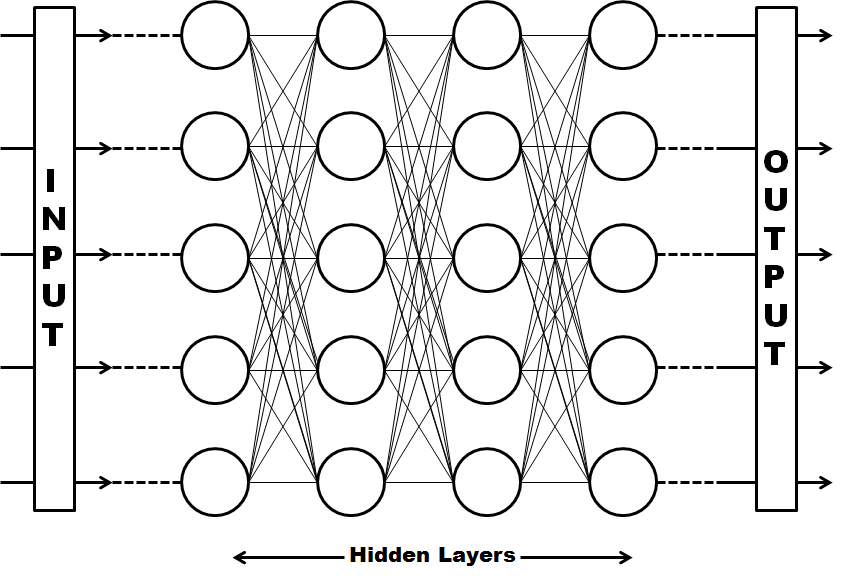
\includegraphics[scale=0.60]{Images/nn_simple_dep}
	\caption{\label{fig:nn_simple_dep} A Simple Neural Network} 
\end{figure}


Considering all these background the \textbf{Training Life Cycle} of DNN's has 3 main stages as shown in Figure~\ref{fig:dnn_lifecycle}

\begin{enumerate}
	\item Choosing network structure
	\item Selection of hyper parameters and training algorithm
	\item Network updates during training and stopping criterion
\end{enumerate}

\begin{figure}
	\centering
	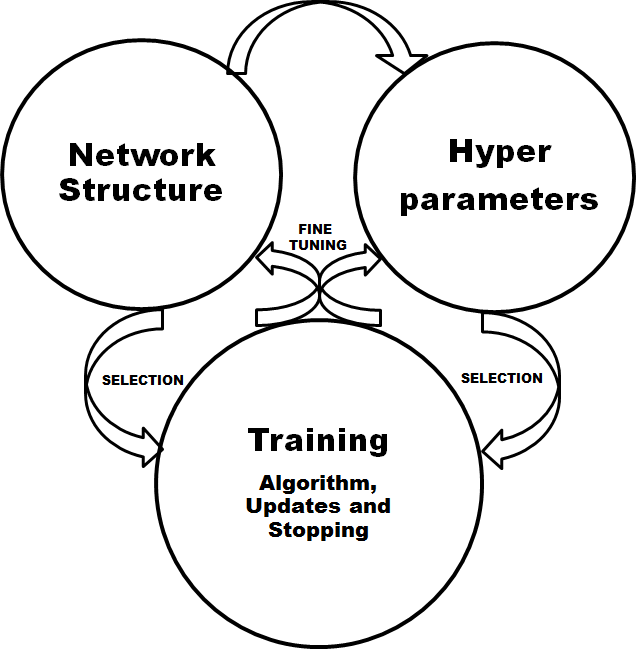
\includegraphics[scale=0.60]{Images/dnn_training_lifecycle}
	\caption{\label{fig:dnn_lifecycle} DNN Training Lifecycle} 
\end{figure}
\section{Chapters Organization}
This study is divided into 6 chapters, Chapter 2, discusses \textbf{Network architecture}, Chapter 3 discusses \textbf{Hyper-parameters}, Chapter 4 discusses \textbf{Training the Network}, Chapter 5 discusses the \textbf{Insights and Recommendations} from this study. Chapter 6 \textbf{concludes} and poses some \textbf{open questions} for future work.

\subsection{Network types}
Chapter \ref{chap:nwstruct} details different architectures, which can be seen as small survey on the state of the art networks used in deep learning.We will keep them for study purposes.

As we studied the details and interdependencies among the training parameters,so we have used our own network, we call it \textbf{ GsNet}. We recommend to use them for comparative study of this kind.
Table \ref{tab:gsnet} shows the layers configuration of GsNet-2,GsNet-3 and GsNet-5.
\begin{table}[!htbp]
	\centering
	\caption{\textbf{GsNet architectures}}
	\label{tab:gsnet}
	\vspace{2mm}
	\begin{tabular}{|l|l|l|}
		\hline
		\hline
		\textbf{GsNet-2} & \textbf{GsNet-3} & \textbf{GsNet-5} 		\\
		\hline
		\hline
		conv 3x3x64 & conv 3x3x64 	& conv 3x3x64 		\\
		pool 2x2    & pool 2x2 		& pool 2x2			\\
		\hline 
		conv 3x3x64 & conv 3x3x64 	& conv 3x3x64 		\\
		pool 2x2    & pool 2x2 		& pool 2x2 			\\
		\hline
		
		& conv 3x3x64 	& conv 3x3x64 		\\
		& pool 2x2 		& pool 2x2 			\\
		\hline
		&        		& conv 3x3x64 		\\
		&  				& pool 2x2 			\\
		\hline
		&  				& conv 3x3x64 		\\
		&  				& pool 2x2 			\\
		\hline
		dense,128 	& dense,128 	& dense,128  		\\
		\hline
		softmax,c 	& softmax,c 	& softmax,c  		\\
		\hline
		\hline
	\end{tabular}
\end{table}

We have used these networks for our experiments and their analysis. This may bring how depth affects learning. Different architectures in practice are described, which can be seen as small survey on state of the art network architectures in chapter \ref{chap:nwstruct}.

\subsection{Hyper-parameters}
Hyper-parameters are discussed in chapter \ref{chap:hyperparams}.Main parameters, which we studied are as following
\begin{enumerate}
	\item Batch Size
	\item Optimizations
	\item Initializations
\end{enumerate} 

Firstly we describe all the different prescribed available techniques for these parameters which can be seen as a small survey of the available studies, experimental results and techniques.

Secondly we present results of almost exhaustive set of parameters configuration. Then best of parameters and configurations are chosen for the next set of experiments.

\subsection{Training the network}

Chapter \ref{chap:training} discusses training the network and study which describes different techniques used in training.We will also explain our training set up which is used for our experiments.


\subsection{Insights and Recommendations}
Chapter \ref{chap:recommendations} provides all insights and analysis of our results. This includes well performing strategies as well as strategies which may didn't  perform well.
Based on these we will describe our recommendations. Also we will explain novel technique which perform well and provide more stability to the learning system.

\subsection{Conclusion}
Chapter \ref{chap:conclusions} concludes with the summary of our study and future direction of this work.

%\iffalse
\section{Notations used}
This section explains the notations used through out this study.
\subsection{DNN Setting}
DNN goal is to approximate a target function $g^*$ for the unknown distribution input $X^*=(x_1,x_2,......x_d)^T \in \mathbb{R}^d$. The target value is $Y^*=(y_1,y_2,........y_s) \in \mathbb{R}^s$. if $\theta^*$ is the parameters associated, then 
\begin{equation}
Y^*=g^*(X^*, \theta^*)
\end{equation}								

$X^*$ represents entire input data for the underlying input distribution. 
Getting $X^*$ is almost impossible, so generally $g^*$ is approximate using the representative input $X$ of size $N$ which is sampled from $X^*$ and hoped to have same distribution as the original input distribution. Let $Y$ is the target value for $X$.

So DNN problem reduces to approximating $ g^*$ using $(X,Y)$ of size $N$. $\theta=(\theta_1,\theta_2...\theta_m) \in \mathbb{R}^m$ represents the parameters which gives best approximation for target function. Finally the DNN has to learn the best $\theta$  such that $g(X,\theta) \sim g^*$. 

$g$ represents a chained function in context of DNN as it flows from input to output via hidden layers as shown in \ref{fig:nn_simple_dep}. $g$ as chained function flowing via hidden layers can  be written as
\begin{equation}
g(X)=g^K(g^{K-1}(g^{K-2}......(g^2(g^1(X))).......)) 
\end{equation}
where $K$ represents total number of hidden layers and $\{g^k, k=1....K\}$ is output of $k^{th}$ layer.Let $\hat{Y}=g(X)$ then lets define a loss function $\mathcal{L}(\hat{Y},Y)$ as the cost it incurs using $g(X)$ to approximate $g^*(X)$ and hence it is also known as cost function.

The gradient of $\mathcal{L}$ with respect to $\theta$ is denoted as $\nabla_{\theta_{t}}\mathcal{L}(\theta_{t})$ at $t^{th}$ iteration. For simplicity we denote this as $\nabla_{\theta_{t}}$, where $\theta_{t}$ denotes the network parameters at iteration/time $t$.

\paragraph{Network Parameters}
%\fi
%\section{Results}
First we will see results related to different database and parameters configurations.
\begin{figure}[H]
	\hspace{-1cm}
	\begin{tabular}{C{.48\textwidth}C{.48\textwidth}}
		%%%%%%%%%%%%%%%%%%%%%% 1 %%%%%%%%%%%%%%%%%%%%%%%%%%%%%%%%%%%
		\subfigure [Training accuracy] {
			\begin{tikzpicture} %
			\begin{axis}[smooth,
			legend pos = south east,
			xlabel={$epochs$}, %
			ylabel={$accuracy$}, %
			mark repeat=10,%
			cycle list/Dark2,
			xticklabel style={/pgf/number format/.cd,fixed,precision=2},%
			%width=0.25
			] %
			\addplot table[x expr=\coordindex , y={acc}, col sep=comma] {Results/cifar100_ThreeLayer_100B_0E_adamax_he_u.csv};
			\addlegendentry{minibatch};%				
			\addplot table[x expr=\coordindex , y={acc}, col sep=comma] {Results/cifar100_carebatch_ThreeLayer_100B_0E_adamax_he_u.csv};
			\addlegendentry{minibatch+care};
			\end{axis} %
			\end{tikzpicture}
		}&
		\subfigure [Validation Accuracy] {
			\begin{tikzpicture} %
			\begin{axis}[smooth,
			legend pos = south east,
			xlabel={$epochs$}, %
			ylabel={$accuracy$}, %
			mark repeat=10,%
			cycle list/Dark2,
			xticklabel style={/pgf/number format/.cd,fixed,precision=2},%
			%width=0.25
			] %
			\addplot table[x expr=\coordindex , y={val_acc}, col sep=comma] {Results/cifar100_ThreeLayer_100B_0E_adamax_he_u.csv};
			\addlegendentry{minibatch};%				
			\addplot table[x expr=\coordindex , y={val_acc}, col sep=comma] {Results/cifar100_carebatch_ThreeLayer_100B_0E_adamax_he_u.csv};
			\addlegendentry{minibatch+care};
			\end{axis} %
			\end{tikzpicture}
		} \\
		\subfigure [Training loss] {
			\begin{tikzpicture} %
			\begin{axis}[smooth,
			xlabel={$epochs$}, %
			ylabel={$error$}, %
			mark repeat=10,%
			cycle list/Dark2,
			xticklabel style={/pgf/number format/.cd,fixed,precision=2},
			] %
			\addplot table[x expr=\coordindex , y={loss}, col sep=comma] {Results/cifar100_ThreeLayer_100B_0E_adamax_he_u.csv};
			\addlegendentry{minibatch};%			
			\addplot table[x expr=\coordindex , y={loss}, col sep=comma] {Results/cifar100_carebatch_ThreeLayer_100B_0E_adamax_he_u.csv};
			\addlegendentry{minibatch+care};
			\end{axis} %
			\end{tikzpicture}
		}&
		\subfigure [Validation loss] {
			\begin{tikzpicture} %
			\begin{axis}[smooth,
			xlabel={$epochs$}, %
			ylabel={$error$}, %
			mark repeat=10,%
			cycle list/Dark2,
			xticklabel style={/pgf/number format/.cd,fixed,precision=2},
			] %
			\addplot table[x expr=\coordindex , y={val_loss}, col sep=comma] {Results/cifar100_ThreeLayer_100B_0E_adamax_he_u.csv};
			\addlegendentry{minibatch};%			
			\addplot table[x expr=\coordindex , y={val_loss}, col sep=comma] {Results/cifar100_carebatch_ThreeLayer_100B_0E_adamax_he_u.csv};
			\addlegendentry{minibatch+care};
			\end{axis} %
			\end{tikzpicture}
		}
	\end{tabular}
	\caption {\textit{hessian uniform,batch size=100,three layer}}
\end{figure}

\begin{figure}[H]
	\hspace{-1cm}
	\begin{tabular}{C{.48\textwidth}C{.48\textwidth}}
		%%%%%%%%%%%%%%%%%%%%%% 1 %%%%%%%%%%%%%%%%%%%%%%%%%%%%%%%%%%%
		\subfigure [Training accuracy] {
			\begin{tikzpicture} %
			\begin{axis}[smooth,
			legend pos = south east,
			xlabel={$epochs$}, %
			ylabel={$accuracy$}, %
			mark repeat=10,%
			cycle list/Dark2,
			xticklabel style={/pgf/number format/.cd,fixed,precision=2},%
			%width=0.25
			] %
			\addplot table[x expr=\coordindex , y={acc}, col sep=comma] {Results/cifar100_FiveLayer_100B_0E_adamax_gl_u.csv};
			\addlegendentry{minibatch};%				
			\addplot table[x expr=\coordindex , y={acc}, col sep=comma] {Results/cifar100_carebatch_FiveLayer_100B_0E_adamax_gl_u.csv};
			\addlegendentry{minibatch+care};
			\end{axis} %
			\end{tikzpicture}
		}&
		\subfigure [Validation Accuracy] {
			\begin{tikzpicture} %
			\begin{axis}[smooth,
			legend pos = south east,
			xlabel={$epochs$}, %
			ylabel={$accuracy$}, %
			mark repeat=10,%
			cycle list/Dark2,
			xticklabel style={/pgf/number format/.cd,fixed,precision=2},%
			%width=0.25
			] %
			\addplot table[x expr=\coordindex , y={val_acc}, col sep=comma] {Results/cifar100_FiveLayer_100B_0E_adamax_gl_u.csv};
			\addlegendentry{minibatch};%				
			\addplot table[x expr=\coordindex , y={val_acc}, col sep=comma] {Results/cifar100_carebatch_FiveLayer_100B_0E_adamax_gl_u.csv};
			\addlegendentry{minibatch+care};
			\end{axis} %
			\end{tikzpicture}
		} \\
		\subfigure [Training loss] {
			\begin{tikzpicture} %
			\begin{axis}[smooth,
			xlabel={$epochs$}, %
			ylabel={$error$}, %
			mark repeat=10,%
			cycle list/Dark2,
			xticklabel style={/pgf/number format/.cd,fixed,precision=2},
			] %
			\addplot table[x expr=\coordindex , y={loss}, col sep=comma] {Results/cifar100_FiveLayer_100B_0E_adamax_gl_u.csv};
			\addlegendentry{minibatch};%			
			\addplot table[x expr=\coordindex , y={loss}, col sep=comma] {Results/cifar100_carebatch_FiveLayer_100B_0E_adamax_gl_u.csv};
			\addlegendentry{minibatch+care};
			\end{axis} %
			\end{tikzpicture}
		}&
		\subfigure [Validation loss] {
			\begin{tikzpicture} %
			\begin{axis}[smooth,
			xlabel={$epochs$}, %
			ylabel={$error$}, %
			mark repeat=10,%
			xticklabel style={/pgf/number format/.cd,fixed,precision=2},
			] %
			\addplot table[x expr=\coordindex , y={val_loss}, col sep=comma] {Results/cifar100_FiveLayer_100B_0E_adamax_gl_u.csv};
			\addlegendentry{minibatch};%			
			\addplot table[x expr=\coordindex , y={val_loss}, col sep=comma] {Results/cifar100_carebatch_FiveLayer_100B_0E_adamax_gl_u.csv};
			\addlegendentry{minibatch+care};
			\end{axis} %
			\end{tikzpicture}
		}
	\end{tabular}
	\caption {\textit{glorot uniform,batch size=100,five layer}}
\end{figure}

\begin{figure}[H]
	\hspace{-1cm}
	\begin{tabular}{C{.48\textwidth}C{.48\textwidth}}
		%%%%%%%%%%%%%%%%%%%%%% 1 %%%%%%%%%%%%%%%%%%%%%%%%%%%%%%%%%%%
		\subfigure [Training accuracy] {
			\begin{tikzpicture} %
			\begin{axis}[smooth,
			legend pos = south east,
			xlabel={$epochs$}, %
			ylabel={$accuracy$}, %
			mark repeat=10,%
			xticklabel style={/pgf/number format/.cd,fixed,precision=2},%
			%width=0.25
			] %
			\addplot table[x expr=\coordindex , y={acc}, col sep=comma] {Results/cifar100_ThreeLayer_100B_0E_adamax_gl_u.csv};
			\addlegendentry{minibatch};%				
			\addplot table[x expr=\coordindex , y={acc}, col sep=comma] {Results/cifar100_carebatch_ThreeLayer_100B_0E_adamax_gl_u.csv};
			\addlegendentry{minibatch+care};
			\end{axis} %
			\end{tikzpicture}
		}&
		\subfigure [Validation Accuracy] {
			\begin{tikzpicture} %
			\begin{axis}[smooth,
			legend pos = south east,
			xlabel={$epochs$}, %
			ylabel={$accuracy$}, %
			mark repeat=10,%
			cycle list/Dark2,
			xticklabel style={/pgf/number format/.cd,fixed,precision=2},%
			%width=0.25
			] %
			\addplot table[x expr=\coordindex , y={val_acc}, col sep=comma] {Results/cifar100_ThreeLayer_100B_0E_adamax_gl_u.csv};
			\addlegendentry{minibatch};%				
			\addplot table[x expr=\coordindex , y={val_acc}, col sep=comma] {Results/cifar100_carebatch_ThreeLayer_100B_0E_adamax_gl_u.csv};
			\addlegendentry{minibatch+care};
			\end{axis} %
			\end{tikzpicture}
		} \\
		\subfigure [Training loss] {
			\begin{tikzpicture} %
			\begin{axis}[smooth,
			xlabel={$epochs$}, %
			ylabel={$error$}, %
			mark repeat=10,%
			cycle list/Dark2,
			xticklabel style={/pgf/number format/.cd,fixed,precision=2},
			] %
			\addplot table[x expr=\coordindex , y={loss}, col sep=comma] {Results/cifar100_ThreeLayer_100B_0E_adamax_gl_u.csv};
			\addlegendentry{minibatch};%			
			\addplot table[x expr=\coordindex , y={loss}, col sep=comma] {Results/cifar100_carebatch_ThreeLayer_100B_0E_adamax_gl_u.csv};
			\addlegendentry{minibatch+care};
			\end{axis} %
			\end{tikzpicture}
		}&
		\subfigure [Validation loss] {
			\begin{tikzpicture} %
			\begin{axis}[smooth,
			xlabel={$epochs$}, %
			ylabel={$error$}, %
			mark repeat=10,%
			cycle list/Dark2,
			xticklabel style={/pgf/number format/.cd,fixed,precision=2},
			] %
			\addplot table[x expr=\coordindex , y={val_loss}, col sep=comma] {Results/cifar100_ThreeLayer_100B_0E_adamax_gl_u.csv};
			\addlegendentry{minibatch};%			
			\addplot table[x expr=\coordindex , y={val_loss}, col sep=comma] {Results/cifar100_carebatch_ThreeLayer_100B_0E_adamax_gl_u.csv};
			\addlegendentry{minibatch+care};
			\end{axis} %
			\end{tikzpicture}
		}
	\end{tabular}
	\caption {\textit{glorot uniform,batch size=100,three layer}}
\end{figure}

\begin{figure}[H]
	\hspace{-1cm}
	\begin{tabular}{C{.48\textwidth}C{.48\textwidth}}
		%%%%%%%%%%%%%%%%%%%%%% 1 %%%%%%%%%%%%%%%%%%%%%%%%%%%%%%%%%%%
		\subfigure [Training accuracy] {
			\begin{tikzpicture} %
			\begin{axis}[smooth,
			legend pos = south east,
			xlabel={$epochs$}, %
			ylabel={$accuracy$}, %
			mark repeat=10,%
			cycle list/Dark2,
			xticklabel style={/pgf/number format/.cd,fixed,precision=2},%
			%width=0.25
			] %
			\addplot table[x expr=\coordindex , y={acc}, col sep=comma] {Results/cifar100_FiveLayer_100B_0E_adamax_gl_u.csv};
			\addlegendentry{minibatch};%				
			\addplot table[x expr=\coordindex , y={acc}, col sep=comma] {Results/cifar100_carebatch_FiveLayer_100B_0E_adamax_gl_u.csv};
			\addlegendentry{minibatch+care};
			\end{axis} %
			\end{tikzpicture}
		}&
		\subfigure [Validation Accuracy] {
			\begin{tikzpicture} %
			\begin{axis}[smooth,
			legend pos = south east,
			xlabel={$epochs$}, %
			ylabel={$accuracy$}, %
			mark repeat=10,%
			cycle list/Dark2,
			xticklabel style={/pgf/number format/.cd,fixed,precision=2},%
			%width=0.25
			] %
			\addplot table[x expr=\coordindex , y={val_acc}, col sep=comma] {Results/cifar100_FiveLayer_100B_0E_adamax_gl_u.csv};
			\addlegendentry{minibatch};%				
			\addplot table[x expr=\coordindex , y={val_acc}, col sep=comma] {Results/cifar100_carebatch_FiveLayer_100B_0E_adamax_gl_u.csv};
			\addlegendentry{minibatch+care};
			\end{axis} %
			\end{tikzpicture}
		} \\
		\subfigure [Training loss] {
			\begin{tikzpicture} %
			\begin{axis}[smooth,
			xlabel={$epochs$}, %
			ylabel={$error$}, %
			mark repeat=10,%
			cycle list/Dark2,
			xticklabel style={/pgf/number format/.cd,fixed,precision=2},
			] %
			\addplot table[x expr=\coordindex , y={loss}, col sep=comma] {Results/cifar100_FiveLayer_100B_0E_adamax_gl_u.csv};
			\addlegendentry{minibatch};%			
			\addplot table[x expr=\coordindex , y={loss}, col sep=comma] {Results/cifar100_carebatch_FiveLayer_100B_0E_adamax_gl_u.csv};
			\addlegendentry{minibatch+care};
			\end{axis} %
			\end{tikzpicture}
		}&
		\subfigure [Validation loss] {
			\begin{tikzpicture} %
			\begin{axis}[smooth,
			xlabel={$epochs$}, %
			ylabel={$error$}, %
			mark repeat=10,%
			cycle list/Dark2,
			xticklabel style={/pgf/number format/.cd,fixed,precision=2},
			] %
			\addplot table[x expr=\coordindex , y={val_loss}, col sep=comma] {Results/cifar100_FiveLayer_100B_0E_adamax_gl_u.csv};
			\addlegendentry{minibatch};%			
			\addplot table[x expr=\coordindex , y={val_loss}, col sep=comma] {Results/cifar100_carebatch_FiveLayer_100B_0E_adamax_gl_u.csv};
			\addlegendentry{minibatch+care};
			\end{axis} %
			\end{tikzpicture}
		}
	\end{tabular}
	\caption {\textit{glorot uniform,batch size=100,five layer}}
\end{figure}


	\begin{figure}[H]
		\hspace{-1cm}
		\begin{tabular}{C{.48\textwidth}C{.48\textwidth}}
			%%%%%%%%%%%%%%%%%%%%%% 1 %%%%%%%%%%%%%%%%%%%%%%%%%%%%%%%%%%%
			\subfigure [Training accuracy] {
				\begin{tikzpicture} %
				\begin{axis}[smooth,
				legend pos = south east,
				xlabel={$epochs$}, %
				ylabel={$accuracy$}, %
				mark repeat=10,%
				xticklabel style={/pgf/number format/.cd,fixed,precision=2},
				] %
				\addplot table[x expr=\coordindex , y={acc}, col sep=comma] {Results/cifar100_ThreeLayer_100B_0E_adamax_gl_u.csv};
				\addlegendentry{Three Layer};%				
				\addplot table[x expr=\coordindex , y={acc}, col sep=comma] {Results/cifar100_FiveLayer_100B_0E_adamax_gl_u.csv};
				\addlegendentry{Five Layer};
				\end{axis} %
				\end{tikzpicture}
			}&
			\subfigure [Validation accuracy] {
				\begin{tikzpicture} %
				\begin{axis}[smooth,
				legend pos = south east,
				xlabel={$epochs$}, %
				mark repeat=10,%
				xticklabel style={/pgf/number format/.cd,fixed,precision=2},
				] %
				\addplot table[x expr=\coordindex , y={val_acc}, col sep=comma] {Results/cifar100_ThreeLayer_100B_0E_adamax_gl_u.csv};
				\addlegendentry{Three Layer};%				
				\addplot table[x expr=\coordindex , y={val_acc}, col sep=comma] {Results/cifar100_FiveLayer_100B_0E_adamax_gl_u.csv};
				\addlegendentry{Five Layer};
				\end{axis} %
				\end{tikzpicture}
			} \\
			\subfigure [Training loss] {
				\begin{tikzpicture} %
				\begin{axis}[smooth,
				xlabel={$epochs$}, %
				ylabel={$error$}, %
				mark repeat=10,%
				xticklabel style={/pgf/number format/.cd,fixed,precision=2},
				] %
				\addplot table[x expr=\coordindex , y={loss}, col sep=comma] {Results/cifar100_ThreeLayer_100B_0E_adamax_gl_u.csv};
				\addlegendentry{Three Layer};%				
				\addplot table[x expr=\coordindex , y={loss}, col sep=comma] {Results/cifar100_FiveLayer_100B_0E_adamax_gl_u.csv};
				\addlegendentry{Five Layer};
				\end{axis} %
				\end{tikzpicture}
			}&
			\subfigure [Validation loss] {
				\begin{tikzpicture} %
				\begin{axis}[smooth,
				xlabel={$epochs$}, %
				mark repeat=10,%
				xticklabel style={/pgf/number format/.cd,fixed,precision=2},
				] %
				\addplot table[x expr=\coordindex , y={val_loss}, col sep=comma] {Results/cifar100_ThreeLayer_100B_0E_adamax_gl_u.csv};
				\addlegendentry{Three Layer};%				
				\addplot table[x expr=\coordindex , y={val_loss}, col sep=comma] {Results/cifar100_FiveLayer_100B_0E_adamax_gl_u.csv};
				\addlegendentry{Five Layer};
				\end{axis} %
				\end{tikzpicture}
			}
		\end{tabular}
		\caption {\textit{optimizer=adamax, initializer=glorot uniform and batch size=100}}
	\end{figure}
	
	\begin{figure}[H]
		\hspace{-1cm}
		\begin{tabular}{C{.48\textwidth}C{.48\textwidth}}
			%%%%%%%%%%%%%%%%%%%%%% 1 %%%%%%%%%%%%%%%%%%%%%%%%%%%%%%%%%%%
			\subfigure [Training accuracy] {
				\begin{tikzpicture} %
				\begin{axis}[smooth,
				legend pos = south east,
				xlabel={$epochs$}, %
				ylabel={$accuracy$}, %
				mark repeat=10,%
				cycle list/Dark2,
				xticklabel style={/pgf/number format/.cd,fixed,precision=2},
				] %
				\addplot table[x expr=\coordindex , y={acc}, col sep=comma] {Results/cifar100_ThreeLayer_100B_0E_adamax_he_u.csv};
				\addlegendentry{Three Layer};%				
				\addplot table[x expr=\coordindex , y={acc}, col sep=comma] {Results/cifar100_FiveLayer_100B_0E_adamax_he_u.csv};
				\addlegendentry{Five Layer};
				\end{axis} %
				\end{tikzpicture}
			}&
			\subfigure [Validation accuracy] {
				\begin{tikzpicture} %
				\begin{axis}[smooth,
				legend pos = south east,
				xlabel={$epochs$}, %
				mark repeat=10,%
				cycle list/Dark2,
				xticklabel style={/pgf/number format/.cd,fixed,precision=2},
				] %
				\addplot table[x expr=\coordindex , y={val_acc}, col sep=comma] {Results/cifar100_ThreeLayer_100B_0E_adamax_he_u.csv};
				\addlegendentry{Three Layer};%				
				\addplot table[x expr=\coordindex , y={val_acc}, col sep=comma] {Results/cifar100_FiveLayer_100B_0E_adamax_he_u.csv};
				\addlegendentry{Five Layer};
				\end{axis} %
				\end{tikzpicture}
			} \\
			\subfigure [Training loss] {
				\begin{tikzpicture} %
				\begin{axis}[smooth,
				xlabel={$epochs$}, %
				ylabel={$error$}, %
				%mark repeat=10,%
				cycle list/Dark2,
				xticklabel style={/pgf/number format/.cd,fixed,precision=2},
				] %
				\addplot table[x expr=\coordindex , y={loss}, col sep=comma] {Results/cifar100_ThreeLayer_100B_0E_adamax_gl_u.csv};
				\addlegendentry{Three Layer};%				
				\addplot table[x expr=\coordindex , y={loss}, col sep=comma] {Results/cifar100_FiveLayer_100B_0E_adamax_gl_u.csv};
				\addlegendentry{Five Layer};
				\end{axis} %
				\end{tikzpicture}
			}&
			\subfigure [Validation loss] {
				\begin{tikzpicture} %
				\begin{axis}[smooth,
				xlabel={$epochs$}, %
				mark repeat=10,%
				cycle list/Dark2,
				xticklabel style={/pgf/number format/.cd,fixed,precision=2},
				] %
				\addplot table[x expr=\coordindex , y={val_loss}, col sep=comma] {Results/cifar100_ThreeLayer_100B_0E_adamax_gl_u.csv};
				\addlegendentry{Three Layer};%				
				\addplot table[x expr=\coordindex , y={val_loss}, col sep=comma] {Results/cifar100_FiveLayer_100B_0E_adamax_gl_u.csv};
				\addlegendentry{Five Layer};
				\end{axis} %
				\end{tikzpicture}
			}
		\end{tabular}
		\caption {\textit{optimizer=adamax, initializer=hessian uniform and batch size=100}}
	\end{figure}


%\section{MNIST Results}
First we will see results related to different database and parameters configurations.


\begin{figure}[H]
	\hspace{-1cm}
			\begin{tikzpicture} %
			\begin{axis}[smooth,
			legend pos = north east,
			mark repeat=10,%
			] %
			\addplot3 [surf,z buffer=sort, mesh/rows=5, shader=interp]
			table[y={batch}, x={index} , z={val_loss}, col sep=comma] {ResultsNormal/data.csv};
			\end{axis} %
			\end{tikzpicture}
	\end{figure}


%%%%%%%%%%%%%%%%%%%%%%%%%%%%%%%%%%%%START: BATCH DEPENDENCIES RESULTS%%%%%%%%%%%%%%%%%%%%%%%%%%%%%%%

\begin{figure}[H]
	\hspace{-1cm}
	\begin{tabular}{C{.48\textwidth}C{.48\textwidth}}
		%%%%%%%%%%%%%%%%%%%%%% 1 %%%%%%%%%%%%%%%%%%%%%%%%%%%%%%%%%%%
		\subfigure [Five layer, adagrad, hessian uniform] {
			\begin{tikzpicture} %
			\begin{axis}[smooth,
			legend pos = north east,
			mark repeat=10,%
			] %
			\addplot3 [surf,draw=red,z buffer=sort, mesh/rows=5]
			table[y={batch}, x={index} , z={val_loss}, col sep=comma] {ResultsNormal/data.csv};
			%\addplot3 [surf]
			%table[y expr=4, x expr=\coordindex , z={val_loss}, col sep=comma] {ResultsNormal/mnist_FiveLayer_40B_0E_adagrad_he_u.csv};
			%\addlegendentry{40};%							
		    %\addplot3 [surf] table[y expr=6, x expr=\coordindex , z={val_loss}, col sep=comma] {ResultsNormal/mnist_FiveLayer_60B_0E_adagrad_he_u.csv};
			%\addlegendentry{20};%	
			%\addplot3 table[y expr=4, x expr=\coordindex , z={val_loss}, col sep=comma] {ResultsNormal/mnist_FiveLayer_40B_0E_adagrad_he_u.csv};
			%\addlegendentry{40};%							
			%\addplot3 table[y expr=6, x expr=\coordindex , z={val_loss}, col sep=comma] {ResultsNormal/mnist_FiveLayer_60B_0E_adagrad_he_u.csv};
			%\addlegendentry{60};%							
			%\addplot3 table[y expr=8, x expr=\coordindex , z={val_loss}, col sep=comma] {ResultsNormal/mnist_FiveLayer_80B_0E_adagrad_he_u.csv};
			%\addlegendentry{80};%							
			%\addplot3 table[y expr=10, x expr=\coordindex , z={val_loss}, col sep=comma] {ResultsNormal/mnist_FiveLayer_100B_0E_adagrad_he_u.csv};
			%\addlegendentry{100};%
			%\addplot3 table[y expr=12, x expr=\coordindex , z={val_loss}, col sep=comma] {ResultsNormal/mnist_FiveLayer_120B_0E_adagrad_he_u.csv};
			%\addlegendentry{120};%							
			%\addplot3 table[y expr=14, x expr=\coordindex , z={val_loss}, col sep=comma] {ResultsNormal/mnist_FiveLayer_140B_0E_adagrad_he_u.csv};
			%\addlegendentry{140};%							
			%\addplot3 table[y expr=16, x expr=\coordindex , z={val_loss}, col sep=comma] {ResultsNormal/mnist_FiveLayer_160B_0E_adagrad_he_u.csv};
			%\addlegendentry{160};%
			%\addplot3 table[y expr=18, x expr=\coordindex , z={val_loss}, col sep=comma] {ResultsNormal/mnist_FiveLayer_180B_0E_adagrad_he_u.csv};
			%\addlegendentry{180};%							
			%\legend{}
			\end{axis} %
			\end{tikzpicture}
		}&
		\subfigure [Three layer, adagrad, hessian uniform] {
			\begin{tikzpicture} %
			\begin{axis}[smooth,
			legend pos = north east,
			xlabel={$epochs$}, %
			zlabel={$error$}, %
			mark repeat=10,%
			% load a color `cycle list' from the `colorbrewer' library
			cycle list/Dark2,
			% define fill color for the marker
			% create new `cycle list` from existing `cycle list's and an
			cycle multiindex* list={
				Dark2
				\nextlist
				my marks
				\nextlist
				[3 of]linestyles
				\nextlist
				solid
				\nextlist
			},
			mark list fill={.!75!white},
			xticklabel style={/pgf/number format/.cd,fixed,precision=2},%
			%width=0.25
			] %
			\addplot3 [fill=orange,fill opacity=0.75,draw=orange!80!black,thick,mark=none] table[y expr=2, x expr=\coordindex , z={val_loss}, col sep=comma] {ResultsNormal/mnist_ThreeLayer_20B_0E_adagrad_he_u.csv};
			\addlegendentry{20};%	
			\addplot3 [fill=yellow,fill opacity=0.55,draw=yellow!80!black,thick,mark=none] table[y expr=4, x expr=\coordindex , z={val_loss}, col sep=comma] {ResultsNormal/mnist_ThreeLayer_40B_0E_adagrad_he_u.csv};
			\addlegendentry{40};%							
			\addplot3 [fill=green,fill opacity=0.55,draw=yellow!80!black,thick,mark=none] table[y expr=6, x expr=\coordindex , z={val_loss}, col sep=comma] {ResultsNormal/mnist_ThreeLayer_60B_0E_adagrad_he_u.csv};
			\addlegendentry{60};%							
			\addplot3 [fill=red,fill opacity=0.55,draw=yellow!80!black,thick,mark=none] table[y expr=8, x expr=\coordindex , z={val_loss}, col sep=comma] {ResultsNormal/mnist_ThreeLayer_80B_0E_adagrad_he_u.csv};
			\addlegendentry{80};%							
			\addplot3 [fill=violet,fill opacity=0.55,draw=yellow!80!black,thick,mark=none] table[y expr=10, x expr=\coordindex , z={val_loss}, col sep=comma] {ResultsNormal/mnist_ThreeLayer_100B_0E_adagrad_he_u.csv};
			\addlegendentry{100};%
			\addplot3 [fill=pink,fill opacity=0.55,draw=yellow!80!black,thick,mark=none] table[y expr=12, x expr=\coordindex , z={val_loss}, col sep=comma] {ResultsNormal/mnist_ThreeLayer_120B_0E_adagrad_he_u.csv};
			\addlegendentry{120};%							
			\addplot3 [fill=orange,fill opacity=0.55,draw=yellow!80!black,thick,mark=none] table[y expr=14, x expr=\coordindex , z={val_loss}, col sep=comma] {ResultsNormal/mnist_ThreeLayer_140B_0E_adagrad_he_u.csv};
			\addlegendentry{140};%							
			\addplot3 [fill=blue,fill opacity=0.55,draw=yellow!80!black,thick,mark=none] table[y expr=16, x expr=\coordindex , z={val_loss}, col sep=comma] {ResultsNormal/mnist_ThreeLayer_160B_0E_adagrad_he_u.csv};
			\addlegendentry{160};%
			\addplot3 [fill=black,fill opacity=0.55,draw=yellow!80!black,thick,mark=none] table[y expr=18, x expr=\coordindex , z={val_loss}, col sep=comma] {ResultsNormal/mnist_ThreeLayer_180B_0E_adagrad_he_u.csv};
			\addlegendentry{180};%							
			\legend{}
			\end{axis} %
			\end{tikzpicture}
		} \\
		\subfigure [Two layer, adagrad, hessian uniform] {
			\begin{tikzpicture} %
			\begin{axis}[smooth,
			legend pos = north east,
			xlabel={$epochs$}, %
			zlabel={$error$}, %
			mark repeat=10,%
			% load a color `cycle list' from the `colorbrewer' library
			cycle list/Dark2,
			% define fill color for the marker
			% create new `cycle list` from existing `cycle list's and an
			cycle multiindex* list={
				Dark2
				\nextlist
				my marks
				\nextlist
				[3 of]linestyles
				\nextlist
				solid
				\nextlist
			},
			mark list fill={.!75!white},
			xticklabel style={/pgf/number format/.cd,fixed,precision=2},%
			%width=0.25
			] %
			\addplot3 [fill=orange,fill opacity=0.75,draw=orange!80!black,thick,mark=none] table[y expr=2, x expr=\coordindex , z={val_loss}, col sep=comma] {ResultsNormal/mnist_TwoLayer_20B_0E_adagrad_he_u.csv};
			\addlegendentry{20};%	
			\addplot3 [fill=yellow,fill opacity=0.55,draw=yellow!80!black,thick,mark=none] table[y expr=4, x expr=\coordindex , z={val_loss}, col sep=comma] {ResultsNormal/mnist_TwoLayer_40B_0E_adagrad_he_u.csv};
			\addlegendentry{40};%							
			\addplot3 [fill=green,fill opacity=0.55,draw=yellow!80!black,thick,mark=none] table[y expr=6, x expr=\coordindex , z={val_loss}, col sep=comma] {ResultsNormal/mnist_TwoLayer_60B_0E_adagrad_he_u.csv};
			\addlegendentry{60};%							
			\addplot3 [fill=red,fill opacity=0.55,draw=yellow!80!black,thick,mark=none] table[y expr=8, x expr=\coordindex , z={val_loss}, col sep=comma] {ResultsNormal/mnist_TwoLayer_80B_0E_adagrad_he_u.csv};
			\addlegendentry{80};%							
			\addplot3 [fill=violet,fill opacity=0.55,draw=yellow!80!black,thick,mark=none] table[y expr=10, x expr=\coordindex , z={val_loss}, col sep=comma] {ResultsNormal/mnist_TwoLayer_100B_0E_adagrad_he_u.csv};
			\addlegendentry{100};%
			\addplot3 [fill=pink,fill opacity=0.55,draw=yellow!80!black,thick,mark=none] table[y expr=12, x expr=\coordindex , z={val_loss}, col sep=comma] {ResultsNormal/mnist_TwoLayer_120B_0E_adagrad_he_u.csv};
			\addlegendentry{120};%							
			\addplot3 [fill=orange,fill opacity=0.55,draw=yellow!80!black,thick,mark=none] table[y expr=14, x expr=\coordindex , z={val_loss}, col sep=comma] {ResultsNormal/mnist_TwoLayer_140B_0E_adagrad_he_u.csv};
			\addlegendentry{140};%							
			\addplot3 [fill=blue,fill opacity=0.55,draw=yellow!80!black,thick,mark=none] table[y expr=16, x expr=\coordindex , z={val_loss}, col sep=comma] {ResultsNormal/mnist_TwoLayer_160B_0E_adagrad_he_u.csv};
			\addlegendentry{160};%
			\addplot3 [fill=black,fill opacity=0.55,draw=yellow!80!black,thick,mark=none] table[y expr=18, x expr=\coordindex , z={val_loss}, col sep=comma] {ResultsNormal/mnist_TwoLayer_180B_0E_adagrad_he_u.csv};
			\addlegendentry{180};%							
			\legend{}
			\end{axis} %
			\end{tikzpicture}
		}&
		\subfigure [Two layer, SGD, hessian uniform] {
			\begin{tikzpicture} %
			\begin{axis}[smooth,
			legend pos = north east,
			xlabel={$epochs$}, %
			zlabel={$error$}, %
			mark repeat=10,%
			% load a color `cycle list' from the `colorbrewer' library
			cycle list/Dark2,
			% define fill color for the marker
			% create new `cycle list` from existing `cycle list's and an
			cycle multiindex* list={
				Dark2
				\nextlist
				my marks
				\nextlist
				[3 of]linestyles
				\nextlist
				solid
				\nextlist
			},
			mark list fill={.!75!white},
			xticklabel style={/pgf/number format/.cd,fixed,precision=2},%
			%width=0.25
			] %
			\addplot3  table[y expr=1, x expr=\coordindex , z={val_loss}, col sep=comma] {ResultsNormal/mnist_TwoLayer_10B_0E_SGD_he_u.csv};
			\addlegendentry{10};%	
			\addplot3  table[y expr=2, x expr=\coordindex , z={val_loss}, col sep=comma] {ResultsNormal/mnist_TwoLayer_20B_0E_SGD_he_u.csv};
			\addlegendentry{20};%	
			\addplot3  table[y expr=4, x expr=\coordindex , z={val_loss}, col sep=comma] {ResultsNormal/mnist_TwoLayer_40B_0E_SGD_he_u.csv};
			\addlegendentry{40};%							
			\addplot3  table[y expr=6, x expr=\coordindex , z={val_loss}, col sep=comma] {ResultsNormal/mnist_TwoLayer_60B_0E_SGD_he_u.csv};
			\addlegendentry{60};%							
			\addplot3  table[y expr=8, x expr=\coordindex , z={val_loss}, col sep=comma] {ResultsNormal/mnist_TwoLayer_80B_0E_SGD_he_u.csv};
			\addlegendentry{80};%							
			\addplot3  table[y expr=10, x expr=\coordindex , z={val_loss}, col sep=comma] {ResultsNormal/mnist_TwoLayer_100B_0E_SGD_he_u.csv};
			\addlegendentry{100};%
			\addplot3  table[y expr=12, x expr=\coordindex , z={val_loss}, col sep=comma] {ResultsNormal/mnist_TwoLayer_120B_0E_SGD_he_u.csv};
			\addlegendentry{120};%							
			\addplot3  table[y expr=14, x expr=\coordindex , z={val_loss}, col sep=comma] {ResultsNormal/mnist_TwoLayer_140B_0E_SGD_he_u.csv};
			\addlegendentry{140};%							
			\addplot3  table[y expr=16, x expr=\coordindex , z={val_loss}, col sep=comma] {ResultsNormal/mnist_TwoLayer_160B_0E_SGD_he_u.csv};
			\addlegendentry{160};%
			\addplot3  table[y expr=18, x expr=\coordindex , z={val_loss}, col sep=comma] {ResultsNormal/mnist_TwoLayer_180B_0E_SGD_he_u.csv};
			\addlegendentry{180};%							
			\legend{}
			\end{axis} %
			\end{tikzpicture}
		}
	\end{tabular}
	\caption {\textit{hessian uniform,batch size=10,three layer}}
\end{figure}

%%%%%%%%%%%%%%%%%%%%%%%%%%%%%%%%%%%%END: BATCH DEPENDENCIES RESULTS%%%%%%%%%%%%%%%%%%%%%%%%%%%%%%%

%%%%%%%%%%%%%%%%%%%%%%%%%%%%%%%%%%%%START VARIOUS STRATEGIES RESULTS%%%%%%%%%%%%%%%%%%%%%%%%%%%%%%%
\begin{figure}[H]
	\hspace{-1cm}
	\begin{tabular}{C{.48\textwidth}C{.48\textwidth}}
		%%%%%%%%%%%%%%%%%%%%%% 1 %%%%%%%%%%%%%%%%%%%%%%%%%%%%%%%%%%%
		\subfigure [Two Layer] {
			\begin{tikzpicture} %
			\begin{axis}[smooth,
			legend pos = north east,
			xlabel={$epochs$}, %
			zlabel={$error$}, %
			mark repeat=10,%
			ymin=1,%
			ymax=3,%
		%	ytick={1,...,3},
		%	yticklabel={outliers,care,minibatch},
			%xmin=100,
			% load a color `cycle list' from the `colorbrewer' library
			cycle list/Dark2,
			% define fill color for the marker
			% create new `cycle list` from existing `cycle list's and an
			cycle multiindex* list={
				Dark2
				\nextlist
				my marks
				\nextlist
				[3 of]linestyles
				\nextlist
				solid
				\nextlist
			},
			mark list fill={.!75!white},
			xticklabel style={/pgf/number format/.cd,fixed,precision=2},%
			%width=0.25
			] %
			\addplot3 [fill=orange,fill opacity=0.75,draw=orange!80!black,thick,mark=none] table[y expr=3, x expr=\coordindex , z={val_loss}, col sep=comma] {Results/mnist_TwoLayer_10B_0E_adamax_he_u.csv};
			\addlegendentry{minibatch};%	
			\addplot3 [fill=yellow,fill opacity=0.55,draw=yellow!80!black,thick,mark=none] table[y expr=2, x expr=\coordindex , z={val_loss}, col sep=comma] {Results/mnist_carebatch_TwoLayer_10B_0E_adamax_gl_u.csv};
			\addlegendentry{care};%							
			\addplot3 [fill=violet,fill opacity=0.50,draw=violet!80!black,thick,mark=none] table[y expr=1, x expr=\coordindex , z={val_loss}, col sep=comma] {Results/outliers_2_1_100_10_1/mnist_iqr_outliers_npass_TwoLayer_10B_0E_adamax_gl_u.csv};
			\addlegendentry{outliers+npass};
			\end{axis} %
			\end{tikzpicture}
		}&
		\subfigure [Three Layer] {
			\begin{tikzpicture} %
			\begin{axis}[smooth,
			legend pos = north east,
			xlabel={$epochs$}, %
			%zlabel={$error$}, %
			mark repeat=10,%
			%xmax=100,%
			% load a color `cycle list' from the `colorbrewer' library
			cycle list/Dark2,
			% define fill color for the marker
			mark list fill={.!75!white},
			% create new `cycle list` from existing `cycle list's and an
			cycle multiindex* list={
				Dark2
				\nextlist
				my marks
				\nextlist
				[3 of]linestyles
				\nextlist
				solid
				\nextlist
			},
			xticklabel style={/pgf/number format/.cd,fixed,precision=2},%
			%width=0.25
			] %
			\addplot3 [fill=orange,fill opacity=0.75,draw=orange!80!black,thick,mark=none]  table[y expr=3, x expr=\coordindex  , z={val_loss}, col sep=comma] {Results/mnist_ThreeLayer_10B_0E_adamax_he_u.csv};
			\addlegendentry{minibatch};%	
			\addplot3 [fill=yellow,fill opacity=0.55,draw=yellow!80!black,thick,mark=none] table[y expr=2, x expr=\coordindex  , z={val_loss}, col sep=comma] {Results/mnist_carebatch_ThreeLayer_10B_0E_adamax_he_u.csv};
			\addlegendentry{care};%	
			\addplot3 [fill=violet,fill opacity=0.50,draw=violet!80!black,thick,mark=none] table[y expr=1, x expr=\coordindex  , z={val_loss}, col sep=comma] {Results/outliers_2_1_100_10_1/mnist_iqr_outliers_npass_ThreeLayer_10B_0E_adamax_he_u.csv};
			\addlegendentry{outliers+npass};
			\end{axis} %
			\end{tikzpicture}
		} \\
		\subfigure [Five Layer] {
			\begin{tikzpicture} %
			\begin{axis}[smooth,
			legend pos = north east,
			xlabel={$epochs$}, %
			zlabel={$error$}, %
			mark repeat=10,%
			% load a color `cycle list' from the `colorbrewer' library
			cycle list/Dark2,
			% define fill color for the marker
			mark list fill={.!75!white},
			xticklabel style={/pgf/number format/.cd,fixed,precision=2},%
			%width=0.25
			] %
			\addplot3 [fill=orange,fill opacity=0.75,draw=orange!80!black,thick,mark=none] table[y expr=3, x expr=\coordindex  , z={val_loss}, col sep=comma] {Results/mnist_FiveLayer_10B_0E_adamax_he_u.csv};
			\addlegendentry{minibatch};%	
			\addplot3 [fill=yellow,fill opacity=0.55,draw=yellow!80!black,thick,mark=none] table[y expr=2, x expr=\coordindex  , z={val_loss}, col sep=comma] {Results/mnist_carebatch_FiveLayer_10B_0E_adamax_he_u.csv};
			\addlegendentry{care};%				
			\addplot3 [fill=violet,fill opacity=0.50,draw=violet!80!black,thick,mark=none] table[y expr=1, x expr=\coordindex  , z={val_loss}, col sep=comma] {Results/outliers_2_1_100_10_1/mnist_iqr_outliers_npass_FiveLayer_10B_0E_adamax_he_u.csv};
			\addlegendentry{outliers+npass};
			\end{axis} %
			\end{tikzpicture}
		}&
		\subfigure [Validation loss] {
			\begin{tikzpicture} %
			\begin{axis}[smooth,
			xlabel={$epochs$}, %
			ylabel={$error$}, %
			mark repeat=10,%
			% load a color `cycle list' from the `colorbrewer' library
			cycle list/RdGy-6,
			% define fill color for the marker
			mark list fill={.!75!white},
			xticklabel style={/pgf/number format/.cd,fixed,precision=2},
			] %
			\addplot table[x expr=\coordindex , y={val_loss}, col sep=comma] {Results/mnist_TwoLayer_10B_0E_adamax_he_u.csv};
			\addlegendentry{minibatch};%			
			\addplot table[x expr=\coordindex , y={val_loss}, col sep=comma] {Results/outliers_2_1_100_10_1/mnist_iqr_outliers_npass_TwoLayer_10B_0E_adamax_gl_u.csv};
			\addlegendentry{minibatch+outliers+npass};
			\end{axis} %
			\end{tikzpicture}
		}
	\end{tabular}
	\caption {\textit{hessian uniform,batch size=10,three layer}}
\end{figure}



\begin{figure}[H]
	\hspace{-1cm}
	\begin{tabular}{C{.48\textwidth}C{.48\textwidth}}
		%%%%%%%%%%%%%%%%%%%%%% 1 %%%%%%%%%%%%%%%%%%%%%%%%%%%%%%%%%%%
		\subfigure [Training accuracy] {
			\begin{tikzpicture} %
			\begin{axis}[smooth,
			legend pos = south east,
			xlabel={$epochs$}, %
			ylabel={$accuracy$}, %
			mark repeat=10,%
			 % load a color `cycle list' from the `colorbrewer' library
			cycle list/RdGy-6,
			% define fill color for the marker
			mark list fill={.!75!white},
			xticklabel style={/pgf/number format/.cd,fixed,precision=2},%
			%width=0.25
			] %
			\addplot3 [fill=orange,fill opacity=0.75,draw=orange!80!black,thick,mark=none] table[y expr=2, x expr=\coordindex , z={acc}, col sep=comma] {Results/mnist_TwoLayer_10B_0E_adamax_he_u.csv};
			\addlegendentry{minibatch};%				
			\addplot3 [fill=violet,fill opacity=0.50,draw=violet!80!black,thick,mark=none] table[y expr=1, x expr=\coordindex , z={acc}, col sep=comma] {Results/outliers_2_1_100_10_1/mnist_iqr_outliers_npass_TwoLayer_10B_0E_adamax_he_u.csv};
			\addlegendentry{outliers+npass};
			\end{axis} %
			\end{tikzpicture}
		}&
		\subfigure [Validation Accuracy] {
			\begin{tikzpicture} %
			\begin{axis}[smooth,
			legend pos = south east,
			xlabel={$epochs$}, %
			ylabel={$accuracy$}, %
			mark repeat=10,%
			 % load a color `cycle list' from the `colorbrewer' library
			cycle list/RdGy-6,
			% define fill color for the marker
			mark list fill={.!75!white},
			xticklabel style={/pgf/number format/.cd,fixed,precision=2},%
			%width=0.25
			] %
			\addplot3 [fill=orange,fill opacity=0.75,draw=orange!80!black,thick,mark=none] table[y expr=2, x expr=\coordindex , z={val_acc}, col sep=comma] {Results/mnist_TwoLayer_10B_0E_adamax_he_u.csv};
			\addlegendentry{minibatch};%				
			\addplot3 [fill=violet,fill opacity=0.50,draw=violet!80!black,thick,mark=none] table[y expr=1, x expr=\coordindex , z={val_acc}, col sep=comma] {Results/outliers_2_1_100_10_1/mnist_iqr_outliers_npass_TwoLayer_10B_0E_adamax_he_u.csv};
			\addlegendentry{minibatch+outliers+npass};
			\end{axis} %
			\end{tikzpicture}
		} \\
		\subfigure [Training loss] {
			\begin{tikzpicture} %
			\begin{axis}[smooth,
			xlabel={$epochs$}, %
			ylabel={$error$}, %
			mark repeat=10,%
			 % load a color `cycle list' from the `colorbrewer' library
			cycle list/RdGy-6,
			% define fill color for the marker
			mark list fill={.!75!white},
			xticklabel style={/pgf/number format/.cd,fixed,precision=2},
			] %
			\addplot3 [fill=orange,fill opacity=0.75,draw=orange!80!black,thick,mark=none] table[y expr=2, x expr=\coordindex , z={loss}, col sep=comma] {Results/mnist_TwoLayer_10B_0E_adamax_he_u.csv};
			\addlegendentry{minibatch};%			
			\addplot3 [fill=violet,fill opacity=0.50,draw=violet!80!black,thick,mark=none] table[y expr=1, x expr=\coordindex , z={loss}, col sep=comma] {Results/outliers_2_1_100_10_1/mnist_iqr_outliers_npass_TwoLayer_10B_0E_adamax_he_u.csv};
			\addlegendentry{minibatch+outliers+npass};
			\end{axis} %
			\end{tikzpicture}
		}&
		\subfigure [Validation loss] {
			\begin{tikzpicture} %
			\begin{axis}[smooth,
			xlabel={$epochs$}, %
			ylabel={$error$}, %
			mark repeat=10,%
			 % load a color `cycle list' from the `colorbrewer' library
			cycle list/RdGy-6,
			% define fill color for the marker
			mark list fill={.!75!white},
			xticklabel style={/pgf/number format/.cd,fixed,precision=2},
			] %
			\addplot3 [fill=orange,fill opacity=0.75,draw=orange!80!black,thick,mark=none] table[y expr=2, x expr=\coordindex , z={val_loss}, col sep=comma] {Results/mnist_TwoLayer_10B_0E_adamax_he_u.csv};
			\addlegendentry{minibatch};%			
			\addplot3 [fill=violet,fill opacity=0.50,draw=violet!80!black,thick,mark=none] table[y expr=1, x expr=\coordindex , z={val_loss}, col sep=comma] {Results/outliers_2_1_100_10_1/mnist_iqr_outliers_npass_TwoLayer_10B_0E_adamax_gl_u.csv};
			\addlegendentry{minibatch+outliers+npass};
			\end{axis} %
			\end{tikzpicture}
		}
	\end{tabular}
	\caption {\textit{hessian uniform,batch size=10,three layer}}
\end{figure}


\begin{figure}[H]
	
	\hspace{-1cm}
	\begin{tabular}{C{.48\textwidth}C{.48\textwidth}}
		%%%%%%%%%%%%%%%%%%%%%% 1 %%%%%%%%%%%%%%%%%%%%%%%%%%%%%%%%%%%
		\subfigure [Training accuracy] {
			\begin{tikzpicture} %
			\begin{axis}[smooth,
			legend pos = south east,
			xlabel={$epochs$}, %
			ylabel={$accuracy$}, %
			mark repeat=10,%
			 % load a color `cycle list' from the `colorbrewer' library
			cycle list/RdGy-6,
			% define fill color for the marker
			mark list fill={.!75!white},
			xticklabel style={/pgf/number format/.cd,fixed,precision=2},%
			%width=0.25
			] %
			\addplot table[x expr=\coordindex , y={acc}, col sep=comma] {Results/mnist_ThreeLayer_10B_0E_adamax_he_u.csv};
			\addlegendentry{minibatch};%				
			\addplot table[x expr=\coordindex , y={acc}, col sep=comma] {Results/outliers_2_1_100_10_1/mnist_iqr_outliers_npass_ThreeLayer_10B_0E_adamax_he_u.csv};
			\addlegendentry{outliers+npass};
			\end{axis} %
			\end{tikzpicture}
		}&
		\subfigure [Validation Accuracy] {
			\begin{tikzpicture} %
			\begin{axis}[smooth,
			legend pos = south east,
			xlabel={$epochs$}, %
			ylabel={$accuracy$}, %
			mark repeat=10,%
			 % load a color `cycle list' from the `colorbrewer' library
			cycle list/RdGy-6,
			% define fill color for the marker
			mark list fill={.!75!white},
			xticklabel style={/pgf/number format/.cd,fixed,precision=2},%
			%width=0.25
			] %
			\addplot table[x expr=\coordindex , y={val_acc}, col sep=comma] {Results/mnist_ThreeLayer_10B_0E_adamax_he_u.csv};
			\addlegendentry{minibatch};%				
			\addplot table[x expr=\coordindex , y={val_acc}, col sep=comma] {Results/outliers_2_1_100_10_1/mnist_iqr_outliers_npass_ThreeLayer_10B_0E_adamax_he_u.csv};
			\addlegendentry{outliers+npass};
			\end{axis} %
			\end{tikzpicture}
		} \\
		\subfigure [Training loss] {
			\begin{tikzpicture} %
			\begin{axis}[smooth,
			 % load a color `cycle list' from the `colorbrewer' library
			cycle list/RdGy-6,
			% define fill color for the marker
			mark list fill={.!75!white},
			% create new `cycle list` from existing `cycle list's and an
			cycle multiindex* list={
				RdGy-6
				\nextlist
				my marks
				\nextlist
				[3 of]linestyles
				\nextlist
				dashed
				\nextlist
			},
			xlabel={$epochs$}, %
			ylabel={$error$}, %
			mark repeat=10,%
			%cycle list name=my black white,%
			xticklabel style={/pgf/number format/.cd,fixed,precision=2},
			] %
			\addplot table[x expr=\coordindex , y={loss}, col sep=comma] {Results/mnist_ThreeLayer_10B_0E_adamax_he_u.csv};
			\addlegendentry{minibatch};%				
			\addplot table[x expr=\coordindex , y={loss}, col sep=comma] {Results/outliers_2_1_100_10_1/mnist_iqr_outliers_npass_ThreeLayer_10B_0E_adamax_he_u.csv};
			\addlegendentry{outliers+npass};
			\end{axis} %
			\end{tikzpicture}
		}&
		\subfigure [Validation loss] {
			\begin{tikzpicture} %
			\begin{axis}[smooth,
			 % load a color `cycle list' from the `colorbrewer' library
			cycle list/RdGy-6,
			% define fill color for the marker
			mark list fill={.!75!white},
			mark repeat=10,
			% create new `cycle list` from existing `cycle list's and an
			cycle multiindex* list={
				RdGy-6
				\nextlist
				my marks
				\nextlist
				[3 of]linestyles
				\nextlist
				dashed
				\nextlist
			},
			xlabel={$epochs$}, %
			ylabel={$error$}, %
			mark repeat=10,%
			%cycle list name=my black white,%
			xticklabel style={/pgf/number format/.cd,fixed,precision=2},
			] %
			\addplot table[x expr=\coordindex , y={val_loss}, col sep=comma] {Results/mnist_ThreeLayer_10B_0E_adamax_he_u.csv};
			\addlegendentry{minibatch};%				
			\addplot table[x expr=\coordindex , y={val_loss}, col sep=comma] {Results/outliers_2_1_100_10_1/mnist_iqr_outliers_npass_ThreeLayer_10B_0E_adamax_he_u.csv};
			\addlegendentry{outliers+npass};
			\end{axis} %
			\end{tikzpicture}
		}
	\end{tabular}
	\caption {\textit{glorot uniform,batch size=10,three layer}}
\end{figure}



\begin{figure}[H]
	\hspace{-1cm}
	\begin{tabular}{C{.48\textwidth}C{.48\textwidth}}
		%%%%%%%%%%%%%%%%%%%%%% 1 %%%%%%%%%%%%%%%%%%%%%%%%%%%%%%%%%%%
		\subfigure [Training accuracy] {
			\begin{tikzpicture} %
			\begin{axis}[smooth,
			legend pos = south east,
			xlabel={$epochs$}, %
			ylabel={$accuracy$}, %
			mark repeat=10,%
			 % load a color `cycle list' from the `colorbrewer' library
			cycle list/RdGy-6,
			% define fill color for the marker
			mark list fill={.!75!white},
			xticklabel style={/pgf/number format/.cd,fixed,precision=2},%
			%width=0.25
			] %
			\addplot table[x expr=\coordindex , y={acc}, col sep=comma] {Results/mnist_TwoLayer_10B_0E_adamax_he_u.csv};
			\addlegendentry{minibatch};%				
			\addplot table[x expr=\coordindex , y={acc}, col sep=comma] {Results/mnist_carebatch_TwoLayer_10B_0E_adamax_gl_u.csv};
			\addlegendentry{care};
			\addplot table[x expr=\coordindex , y={acc}, col sep=comma] {Results/mnist_careup_init_TwoLayer_10B_0E_adamax_he_u.csv};
			\addlegendentry{careinit};
			\addplot table[x expr=\coordindex , y={acc}, col sep=comma] {Results/outliers_2_1_100_10_1/mnist_iqr_outliers_npass_TwoLayer_10B_0E_adamax_he_u.csv};
			\addlegendentry{outliers+npass};
			\end{axis} %
			\end{tikzpicture}
		}&
		\subfigure [Validation Accuracy] {
			\begin{tikzpicture} %
			\begin{axis}[smooth,
			legend pos = south east,
			xlabel={$epochs$}, %
			ylabel={$accuracy$}, %
			mark repeat=10,%
			 % load a color `cycle list' from the `colorbrewer' library
			cycle list/RdGy-6,
			% define fill color for the marker
			mark list fill={.!75!white},
			xticklabel style={/pgf/number format/.cd,fixed,precision=2},%
			%width=0.25
			] %
			\addplot table[x expr=\coordindex , y={val_acc}, col sep=comma] {Results/mnist_TwoLayer_10B_0E_adamax_he_u.csv};
			\addlegendentry{minibatch};%				
			\addplot table[x expr=\coordindex , y={val_acc}, col sep=comma] {Results/mnist_carebatch_TwoLayer_10B_0E_adamax_gl_u.csv};
			\addlegendentry{minibatch+care};
			\addplot table[x expr=\coordindex , y={val_acc}, col sep=comma]
			{Results/mnist_careup_init_TwoLayer_10B_0E_adamax_he_u.csv};
			\addlegendentry{minibatch+careinit};
			\addplot table[x expr=\coordindex , y={val_acc}, col sep=comma] {Results/outliers_2_1_100_10_1/mnist_iqr_outliers_npass_TwoLayer_10B_0E_adamax_gl_u.csv};
		    \addlegendentry{minibatch+outliers+npass};
			\end{axis} %
			\end{tikzpicture}
		} \\
		\subfigure [Training loss] {
			\begin{tikzpicture} %
			\begin{axis}[smooth,
			xlabel={$epochs$}, %
			ylabel={$error$}, %
			mark repeat=10,%
			 % load a color `cycle list' from the `colorbrewer' library
			cycle list/RdGy-6,
			% define fill color for the marker
			mark list fill={.!75!white},
			xticklabel style={/pgf/number format/.cd,fixed,precision=2},
			] %
			\addplot table[x expr=\coordindex , y={loss}, col sep=comma] {Results/mnist_TwoLayer_10B_0E_adamax_he_u.csv};
			\addlegendentry{minibatch};%			
			\addplot table[x expr=\coordindex , y={loss}, col sep=comma] {Results/mnist_carebatch_TwoLayer_10B_0E_adamax_gl_u.csv};
			\addlegendentry{minibatch+care};
			\addplot table[x expr=\coordindex , y={loss}, col sep=comma]
			{Results/mnist_careup_init_TwoLayer_10B_0E_adamax_he_u.csv};
			\addlegendentry{minibatch+careinit};
			\addplot table[x expr=\coordindex , y={loss}, col sep=comma] {Results/outliers_2_1_100_10_1/mnist_iqr_outliers_npass_TwoLayer_10B_0E_adamax_gl_u.csv};
			\addlegendentry{minibatch+outliers+npass};
			\end{axis} %
			\end{tikzpicture}
		}&
		\subfigure [Validation loss] {
			\begin{tikzpicture} %
			\begin{axis}[smooth,
			xlabel={$epochs$}, %
			ylabel={$error$}, %
			mark repeat=10,%
			 % load a color `cycle list' from the `colorbrewer' library
			cycle list/RdGy-6,
			% define fill color for the marker
			mark list fill={.!75!white},
			xticklabel style={/pgf/number format/.cd,fixed,precision=2},
			] %
			\addplot table[x expr=\coordindex , y={val_loss}, col sep=comma] {Results/mnist_TwoLayer_10B_0E_adamax_he_u.csv};
			\addlegendentry{minibatch};%			
			\addplot table[x expr=\coordindex , y={val_loss}, col sep=comma] {Results/mnist_carebatch_TwoLayer_10B_0E_adamax_gl_u.csv};
			\addlegendentry{minibatch+care};
			\addplot table[x expr=\coordindex , y={val_loss}, col sep=comma]
			{Results/mnist_careup_init_TwoLayer_10B_0E_adamax_he_u.csv};
			\addlegendentry{minibatch+careinit};
			\addplot table[x expr=\coordindex , y={val_loss}, col sep=comma] {Results/outliers_2_1_100_10_1/mnist_iqr_outliers_npass_TwoLayer_10B_0E_adamax_gl_u.csv};
			\addlegendentry{minibatch+outliers+npass};
			\end{axis} %
			\end{tikzpicture}
		}
	\end{tabular}
	\caption {\textit{hessian uniform,batch size=10,three layer}}
\end{figure}


\begin{figure}[H]
	
	\hspace{-1cm}
	\begin{tabular}{C{.48\textwidth}C{.48\textwidth}}
		%%%%%%%%%%%%%%%%%%%%%% 1 %%%%%%%%%%%%%%%%%%%%%%%%%%%%%%%%%%%
		\subfigure [Training accuracy] {
			\begin{tikzpicture} %
			\begin{axis}[smooth,
			legend pos = south east,
			xlabel={$epochs$}, %
			ylabel={$accuracy$}, %
			mark repeat=10,%
			 % load a color `cycle list' from the `colorbrewer' library
			cycle list/RdGy-6,
			% define fill color for the marker
			mark list fill={.!75!white},
			xticklabel style={/pgf/number format/.cd,fixed,precision=2},%
			%width=0.25
			] %
			\addplot table[x expr=\coordindex , y={acc}, col sep=comma] {Results/mnist_ThreeLayer_10B_0E_adamax_he_u.csv};
			\addlegendentry{minibatch};%				
			\addplot table[x expr=\coordindex , y={acc}, col sep=comma] {Results/mnist_carebatch_ThreeLayer_10B_0E_adamax_gl_u.csv};
			\addlegendentry{minibatch+care};
			\addplot table[x expr=\coordindex , y={acc}, col sep=comma] {Results/mnist_careup_init_ThreeLayer_10B_0E_adamax_he_u.csv};
			\addlegendentry{minibatch+careinit};
			\addplot table[x expr=\coordindex , y={acc}, col sep=comma] {Results/outliers_2_1_100_10_1/mnist_iqr_outliers_npass_ThreeLayer_10B_0E_adamax_he_u.csv};
			\addlegendentry{outliers+npass};
			\end{axis} %
			\end{tikzpicture}
		}&
		\subfigure [Validation Accuracy] {
			\begin{tikzpicture} %
			\begin{axis}[smooth,
			legend pos = south east,
			xlabel={$epochs$}, %
			ylabel={$accuracy$}, %
			mark repeat=10,%
			 % load a color `cycle list' from the `colorbrewer' library
			cycle list/RdGy-6,
			% define fill color for the marker
			mark list fill={.!75!white},
			xticklabel style={/pgf/number format/.cd,fixed,precision=2},%
			%width=0.25
			] %
			\addplot table[x expr=\coordindex , y={val_acc}, col sep=comma] {Results/mnist_ThreeLayer_10B_0E_adamax_he_u.csv};
			\addlegendentry{minibatch};%				
			\addplot table[x expr=\coordindex , y={val_acc}, col sep=comma] {Results/mnist_carebatch_ThreeLayer_10B_0E_adamax_gl_u.csv};
			\addlegendentry{minibatch+care};
			\addplot table[x expr=\coordindex , y={val_acc}, col sep=comma] {Results/mnist_careup_init_ThreeLayer_10B_0E_adamax_he_u.csv};
			\addlegendentry{minibatch+careinit};
			\addplot table[x expr=\coordindex , y={val_acc}, col sep=comma] {Results/outliers_2_1_100_10_1/mnist_iqr_outliers_npass_ThreeLayer_10B_0E_adamax_he_u.csv};
			\addlegendentry{outliers+npass};
			\end{axis} %
			\end{tikzpicture}
		} \\
		\subfigure [Training loss] {
			\begin{tikzpicture} %
			\begin{axis}[smooth,
			xlabel={$epochs$}, %
			ylabel={$error$}, %
			mark repeat=10,%
			 % load a color `cycle list' from the `colorbrewer' library
			cycle list/RdGy-6,
			% define fill color for the marker
			mark list fill={.!75!white},
			xticklabel style={/pgf/number format/.cd,fixed,precision=2},
			] %
			\addplot table[x expr=\coordindex , y={loss}, col sep=comma] {Results/mnist_ThreeLayer_10B_0E_adamax_he_u.csv};
			\addlegendentry{minibatch};%				
			\addplot table[x expr=\coordindex , y={loss}, col sep=comma] {Results/mnist_carebatch_ThreeLayer_10B_0E_adamax_gl_u.csv};
			\addlegendentry{minibatch+care};
			\addplot table[x expr=\coordindex , y={loss}, col sep=comma] {Results/mnist_careup_init_ThreeLayer_10B_0E_adamax_he_u.csv};
			\addlegendentry{minibatch+careinit};
			\addplot table[x expr=\coordindex , y={loss}, col sep=comma] {Results/outliers_2_1_100_10_1/mnist_iqr_outliers_npass_ThreeLayer_10B_0E_adamax_he_u.csv};
			\addlegendentry{outliers+npass};
			\end{axis} %
			\end{tikzpicture}
		}&
		\subfigure [Validation loss] {
			\begin{tikzpicture} %
			\begin{axis}[smooth,
			xlabel={$epochs$}, %
			ylabel={$error$}, %
			mark repeat=10,%
			 % load a color `cycle list' from the `colorbrewer' library
			cycle list/RdGy-6,
			% define fill color for the marker
			mark list fill={.!75!white},
			xticklabel style={/pgf/number format/.cd,fixed,precision=2},
			] %
			\addplot table[x expr=\coordindex , y={val_loss}, col sep=comma] {Results/mnist_ThreeLayer_10B_0E_adamax_he_u.csv};
			\addlegendentry{minibatch};%				
			\addplot table[x expr=\coordindex , y={val_loss}, col sep=comma] {Results/mnist_carebatch_ThreeLayer_10B_0E_adamax_gl_u.csv};
			\addlegendentry{minibatch+care};
			\addplot table[x expr=\coordindex , y={val_loss}, col sep=comma] {Results/mnist_careup_init_ThreeLayer_10B_0E_adamax_he_u.csv};
			\addlegendentry{minibatch+careinit};
			\addplot table[x expr=\coordindex , y={val_loss}, col sep=comma] {Results/outliers_2_1_100_10_1/mnist_iqr_outliers_npass_ThreeLayer_10B_0E_adamax_he_u.csv};
			\addlegendentry{outliers+npass};
			\end{axis} %
			\end{tikzpicture}
		}
	\end{tabular}
	\caption {\textit{glorot uniform,batch size=10,three layer}}
\end{figure}

\begin{figure}[H]
	\hspace{-1cm}
	\begin{tabular}{C{.48\textwidth}C{.48\textwidth}}
		%%%%%%%%%%%%%%%%%%%%%% 1 %%%%%%%%%%%%%%%%%%%%%%%%%%%%%%%%%%%
		\subfigure [Training accuracy] {
			\begin{tikzpicture} %
			\begin{axis}[smooth,
			legend pos = south east,
			xlabel={$epochs$}, %
			ylabel={$accuracy$}, %
			mark repeat=10,%
			 % load a color `cycle list' from the `colorbrewer' library
			cycle list/RdGy-6,
			% define fill color for the marker
			mark list fill={.!75!white},
			xticklabel style={/pgf/number format/.cd,fixed,precision=2},%
			%width=0.25
			] %
			\addplot table[x expr=\coordindex , y={acc}, col sep=comma] {Results/mnist_FiveLayer_10B_0E_adamax_he_u.csv};
			\addlegendentry{minibatch};%				
			\addplot table[x expr=\coordindex , y={acc}, col sep=comma] {Results/mnist_carebatch_FiveLayer_10B_0E_adamax_gl_u.csv};
			\addlegendentry{minibatch+care};
			\addplot table[x expr=\coordindex , y={acc}, col sep=comma] {Results/mnist_careup_init_FiveLayer_10B_0E_adamax_he_u.csv};
			\addlegendentry{minibatch+careinit};
			\addplot table[x expr=\coordindex , y={acc}, col sep=comma] {Results/outliers_2_1_100_10_1/mnist_iqr_outliers_npass_FiveLayer_10B_0E_adamax_he_u.csv};
			\addlegendentry{outliers+npass};
			\end{axis} %
			\end{tikzpicture}
		}&
		\subfigure [Validation Accuracy] {
			\begin{tikzpicture} %
			\begin{axis}[smooth,
			legend pos = south east,
			xlabel={$epochs$}, %
			ylabel={$accuracy$}, %
			mark repeat=10,%
			 % load a color `cycle list' from the `colorbrewer' library
			cycle list/RdGy-6,
			% define fill color for the marker
			mark list fill={.!75!white},
			xticklabel style={/pgf/number format/.cd,fixed,precision=2},%
			%width=0.25
			] %
			\addplot table[x expr=\coordindex , y={val_acc}, col sep=comma] {Results/mnist_FiveLayer_10B_0E_adamax_he_u.csv};
			\addlegendentry{minibatch};%				
			\addplot table[x expr=\coordindex , y={val_acc}, col sep=comma] {Results/mnist_carebatch_FiveLayer_10B_0E_adamax_gl_u.csv};
			\addlegendentry{minibatch+care};
			\addplot table[x expr=\coordindex , y={val_acc}, col sep=comma] {Results/mnist_careup_init_FiveLayer_10B_0E_adamax_he_u.csv};
			\addlegendentry{minibatch+careinit};
			\addplot table[x expr=\coordindex , y={val_acc}, col sep=comma] {Results/outliers_2_1_100_10_1/mnist_iqr_outliers_npass_FiveLayer_10B_0E_adamax_he_u.csv};
			\addlegendentry{outliers+npass};
			\end{axis} %
			\end{tikzpicture}
		} \\
		\subfigure [Training loss] {
			\begin{tikzpicture} %
			\begin{axis}[smooth,
			xlabel={$epochs$}, %
			ylabel={$error$}, %
			mark repeat=10,%
			 % load a color `cycle list' from the `colorbrewer' library
			cycle list/RdGy-6,
			% define fill color for the marker
			mark list fill={.!75!white},
			xticklabel style={/pgf/number format/.cd,fixed,precision=2},
			] %
			\addplot table[x expr=\coordindex , y={loss}, col sep=comma] {Results/mnist_FiveLayer_10B_0E_adamax_he_u.csv};
			\addlegendentry{minibatch};%				
			\addplot table[x expr=\coordindex , y={loss}, col sep=comma] {Results/mnist_carebatch_FiveLayer_10B_0E_adamax_gl_u.csv};
			\addlegendentry{minibatch+care};
			\addplot table[x expr=\coordindex , y={loss}, col sep=comma] {Results/mnist_careup_init_FiveLayer_10B_0E_adamax_he_u.csv};
			\addlegendentry{minibatch+careinit};
			\addplot table[x expr=\coordindex , y={loss}, col sep=comma] {Results/outliers_2_1_100_10_1/mnist_iqr_outliers_npass_FiveLayer_10B_0E_adamax_he_u.csv};
			\addlegendentry{outliers+npass};
			\end{axis} %
			\end{tikzpicture}
		}&
		\subfigure [Validation loss] {
			\begin{tikzpicture} %
			\begin{axis}[smooth,
			xlabel={$epochs$}, %
			ylabel={$error$}, %
			mark repeat=10,%
			 % load a color `cycle list' from the `colorbrewer' library
			cycle list/RdGy-6,
			% define fill color for the marker
			mark list fill={.!75!white},
			xticklabel style={/pgf/number format/.cd,fixed,precision=2},
			] %
			\addplot table[x expr=\coordindex , y={val_loss}, col sep=comma] {Results/mnist_FiveLayer_10B_0E_adamax_he_u.csv};
			\addlegendentry{minibatch};%				
			\addplot table[x expr=\coordindex , y={val_loss}, col sep=comma] {Results/mnist_carebatch_FiveLayer_10B_0E_adamax_gl_u.csv};
			\addlegendentry{minibatch+care};
			\addplot table[x expr=\coordindex , y={val_loss}, col sep=comma] {Results/mnist_careup_init_FiveLayer_10B_0E_adamax_he_u.csv};
			\addlegendentry{minibatch+careinit};
			\addplot table[x expr=\coordindex , y={val_loss}, col sep=comma] {Results/outliers_2_1_100_10_1/mnist_iqr_outliers_npass_FiveLayer_10B_0E_adamax_he_u.csv};
			\addlegendentry{outliers+npass};
			\end{axis} %
			\end{tikzpicture}
		}
	\end{tabular}
	\caption {\textit{hessian uniform,batch size=10,five layer}}
\end{figure}


	\begin{figure}[H]
		\hspace{-1cm}
		\begin{tabular}{C{.48\textwidth}C{.48\textwidth}}
			%%%%%%%%%%%%%%%%%%%%%% 1 %%%%%%%%%%%%%%%%%%%%%%%%%%%%%%%%%%%
			\subfigure [Training accuracy] {
				\begin{tikzpicture} %
				\begin{axis}[smooth,
				legend pos = south east,
				xlabel={$epochs$}, %
				ylabel={$accuracy$}, %
				mark repeat=10,%
				 % load a color `cycle list' from the `colorbrewer' library
				cycle list/RdGy-6,
				% define fill color for the marker
				mark list fill={.!75!white},
				xticklabel style={/pgf/number format/.cd,fixed,precision=2},
				] %
				\addplot table[x expr=\coordindex , y={acc}, col sep=comma] {Results/mnist_ThreeLayer_10B_0E_adamax_gl_u.csv};
				\addlegendentry{Three Layer};%				
				\addplot table[x expr=\coordindex , y={acc}, col sep=comma] {Results/mnist_FiveLayer_10B_0E_adamax_gl_u.csv};
				\addlegendentry{Five Layer};
				\end{axis} %
				\end{tikzpicture}
			}&
			\subfigure [Validation accuracy] {
				\begin{tikzpicture} %
				\begin{axis}[smooth,
				legend pos = south east,
				xlabel={$epochs$}, %
				mark repeat=10,%
				 % load a color `cycle list' from the `colorbrewer' library
				cycle list/RdGy-6,
				% define fill color for the marker
				mark list fill={.!75!white},
				xticklabel style={/pgf/number format/.cd,fixed,precision=2},
				] %
				\addplot table[x expr=\coordindex , y={val_acc}, col sep=comma] {Results/mnist_ThreeLayer_10B_0E_adamax_gl_u.csv};
				\addlegendentry{Three Layer};%				
				\addplot table[x expr=\coordindex , y={val_acc}, col sep=comma] {Results/mnist_FiveLayer_10B_0E_adamax_gl_u.csv};
				\addlegendentry{Five Layer};
				\end{axis} %
				\end{tikzpicture}
			} \\
			\subfigure [Training loss] {
				\begin{tikzpicture} %
				\begin{axis}[smooth,
				xlabel={$epochs$}, %
				ylabel={$error$}, %
				mark repeat=10,%
				 % load a color `cycle list' from the `colorbrewer' library
				cycle list/RdGy-6,
				% define fill color for the marker
				mark list fill={.!75!white},
				xticklabel style={/pgf/number format/.cd,fixed,precision=2},
				] %
				\addplot table[x expr=\coordindex , y={loss}, col sep=comma] {Results/mnist_ThreeLayer_10B_0E_adamax_gl_u.csv};
				\addlegendentry{Three Layer};%				
				\addplot table[x expr=\coordindex , y={loss}, col sep=comma] {Results/mnist_FiveLayer_10B_0E_adamax_gl_u.csv};
				\addlegendentry{Five Layer};
				\end{axis} %
				\end{tikzpicture}
			}&
			\subfigure [Validation loss] {
				\begin{tikzpicture} %
				\begin{axis}[smooth,
				xlabel={$epochs$}, %
				mark repeat=10,%
				 % load a color `cycle list' from the `colorbrewer' library
				cycle list/RdGy-6,
				% define fill color for the marker
				mark list fill={.!75!white},
				xticklabel style={/pgf/number format/.cd,fixed,precision=2},
				] %
				\addplot table[x expr=\coordindex , y={val_loss}, col sep=comma] {Results/mnist_ThreeLayer_10B_0E_adamax_gl_u.csv};
				\addlegendentry{Three Layer};%				
				\addplot table[x expr=\coordindex , y={val_loss}, col sep=comma] {Results/mnist_FiveLayer_10B_0E_adamax_gl_u.csv};
				\addlegendentry{Five Layer};
				\end{axis} %
				\end{tikzpicture}
			}
		\end{tabular}
		\caption {\textit{optimizer=adamax, initializer=glorot uniform and batch size=10}}
	\end{figure}
	
	\begin{figure}[H]
		\hspace{-1cm}
		\begin{tabular}{C{.48\textwidth}C{.48\textwidth}}
			%%%%%%%%%%%%%%%%%%%%%% 1 %%%%%%%%%%%%%%%%%%%%%%%%%%%%%%%%%%%
			\subfigure [Training accuracy] {
				\begin{tikzpicture} %
				\begin{axis}[smooth,
				legend pos = south east,
				xlabel={$epochs$}, %
				ylabel={$accuracy$}, %
				mark repeat=10,%
				 % load a color `cycle list' from the `colorbrewer' library
				cycle list/RdGy-6,
				% define fill color for the marker
				mark list fill={.!75!white},
				xticklabel style={/pgf/number format/.cd,fixed,precision=2},
				] %
				\addplot table[x expr=\coordindex , y={acc}, col sep=comma] {Results/mnist_ThreeLayer_10B_0E_adamax_he_u.csv};
				\addlegendentry{Three Layer};%				
				\addplot table[x expr=\coordindex , y={acc}, col sep=comma] {Results/mnist_FiveLayer_10B_0E_adamax_he_u.csv};
				\addlegendentry{Five Layer};
				\end{axis} %
				\end{tikzpicture}
			}&
			\subfigure [Validation accuracy] {
				\begin{tikzpicture} %
				\begin{axis}[smooth,
				legend pos = south east,
				xlabel={$epochs$}, %
				mark repeat=10,%
				 % load a color `cycle list' from the `colorbrewer' library
				cycle list/RdGy-6,
				% define fill color for the marker
				mark list fill={.!75!white},
				xticklabel style={/pgf/number format/.cd,fixed,precision=2},
				] %
				\addplot table[x expr=\coordindex , y={val_acc}, col sep=comma] {Results/mnist_ThreeLayer_10B_0E_adamax_he_u.csv};
				\addlegendentry{Three Layer};%				
				\addplot table[x expr=\coordindex , y={val_acc}, col sep=comma] {Results/mnist_FiveLayer_10B_0E_adamax_he_u.csv};
				\addlegendentry{Five Layer};
				\end{axis} %
				\end{tikzpicture}
			} \\
			\subfigure [Training loss] {
				\begin{tikzpicture} %
				\begin{axis}[smooth,
				xlabel={$epochs$}, %
				ylabel={$error$}, %
				%mark repeat=10,%
				 % load a color `cycle list' from the `colorbrewer' library
				cycle list/RdGy-6,
				% define fill color for the marker
				mark list fill={.!75!white},
				xticklabel style={/pgf/number format/.cd,fixed,precision=2},
				] %
				\addplot table[x expr=\coordindex , y={loss}, col sep=comma] {Results/mnist_ThreeLayer_10B_0E_adamax_gl_u.csv};
				\addlegendentry{Three Layer};%				
				\addplot table[x expr=\coordindex , y={loss}, col sep=comma] {Results/mnist_FiveLayer_10B_0E_adamax_gl_u.csv};
				\addlegendentry{Five Layer};
				\end{axis} %
				\end{tikzpicture}
			}&
			\subfigure [Validation loss] {
				\begin{tikzpicture} %
				\begin{axis}[smooth,
				xlabel={$epochs$}, %
				mark repeat=10,%
				 % load a color `cycle list' from the `colorbrewer' library
				cycle list/RdGy-6,
				% define fill color for the marker
				mark list fill={.!75!white},
				xticklabel style={/pgf/number format/.cd,fixed,precision=2},
				] %
				\addplot table[x expr=\coordindex , y={val_loss}, col sep=comma] {Results/mnist_ThreeLayer_10B_0E_adamax_gl_u.csv};
				\addlegendentry{Three Layer};%				
				\addplot table[x expr=\coordindex , y={val_loss}, col sep=comma] {Results/mnist_FiveLayer_10B_0E_adamax_gl_u.csv};
				\addlegendentry{Five Layer};
				\end{axis} %
				\end{tikzpicture}
			}
		\end{tabular}
		\caption {\textit{optimizer=adamax, initializer=hessian uniform and batch size=10}}
	\end{figure}


%\section{Results}
First we will see results related to different database and parameters configurations.
\begin{figure}[H]
	\hspace{-1cm}
	\begin{tabular}{C{.48\textwidth}C{.48\textwidth}}
		%%%%%%%%%%%%%%%%%%%%%% 1 %%%%%%%%%%%%%%%%%%%%%%%%%%%%%%%%%%%
		\subfigure [Training accuracy] {
			\begin{tikzpicture} %
			\begin{axis}[smooth,
			legend pos = south east,
			xlabel={$epochs$}, %
			ylabel={$accuracy$}, %
			mark repeat=10,%
			cycle list/Dark2,
			xticklabel style={/pgf/number format/.cd,fixed,precision=2},%
			%width=0.25
			] %
			\addplot table[x expr=\coordindex , y={acc}, col sep=comma] {Results/cifar100_ThreeLayer_100B_0E_adamax_he_u.csv};
			\addlegendentry{minibatch};%				
			\addplot table[x expr=\coordindex , y={acc}, col sep=comma] {Results/cifar100_carebatch_ThreeLayer_100B_0E_adamax_he_u.csv};
			\addlegendentry{minibatch+care};
			\end{axis} %
			\end{tikzpicture}
		}&
		\subfigure [Validation Accuracy] {
			\begin{tikzpicture} %
			\begin{axis}[smooth,
			legend pos = south east,
			xlabel={$epochs$}, %
			ylabel={$accuracy$}, %
			mark repeat=10,%
			cycle list/Dark2,
			xticklabel style={/pgf/number format/.cd,fixed,precision=2},%
			%width=0.25
			] %
			\addplot table[x expr=\coordindex , y={val_acc}, col sep=comma] {Results/cifar100_ThreeLayer_100B_0E_adamax_he_u.csv};
			\addlegendentry{minibatch};%				
			\addplot table[x expr=\coordindex , y={val_acc}, col sep=comma] {Results/cifar100_carebatch_ThreeLayer_100B_0E_adamax_he_u.csv};
			\addlegendentry{minibatch+care};
			\end{axis} %
			\end{tikzpicture}
		} \\
		\subfigure [Training loss] {
			\begin{tikzpicture} %
			\begin{axis}[smooth,
			xlabel={$epochs$}, %
			ylabel={$error$}, %
			mark repeat=10,%
			cycle list/Dark2,
			xticklabel style={/pgf/number format/.cd,fixed,precision=2},
			] %
			\addplot table[x expr=\coordindex , y={loss}, col sep=comma] {Results/cifar100_ThreeLayer_100B_0E_adamax_he_u.csv};
			\addlegendentry{minibatch};%			
			\addplot table[x expr=\coordindex , y={loss}, col sep=comma] {Results/cifar100_carebatch_ThreeLayer_100B_0E_adamax_he_u.csv};
			\addlegendentry{minibatch+care};
			\end{axis} %
			\end{tikzpicture}
		}&
		\subfigure [Validation loss] {
			\begin{tikzpicture} %
			\begin{axis}[smooth,
			xlabel={$epochs$}, %
			ylabel={$error$}, %
			mark repeat=10,%
			cycle list/Dark2,
			xticklabel style={/pgf/number format/.cd,fixed,precision=2},
			] %
			\addplot table[x expr=\coordindex , y={val_loss}, col sep=comma] {Results/cifar100_ThreeLayer_100B_0E_adamax_he_u.csv};
			\addlegendentry{minibatch};%			
			\addplot table[x expr=\coordindex , y={val_loss}, col sep=comma] {Results/cifar100_carebatch_ThreeLayer_100B_0E_adamax_he_u.csv};
			\addlegendentry{minibatch+care};
			\end{axis} %
			\end{tikzpicture}
		}
	\end{tabular}
	\caption {\textit{hessian uniform,batch size=100,three layer}}
\end{figure}

\begin{figure}[H]
	\hspace{-1cm}
	\begin{tabular}{C{.48\textwidth}C{.48\textwidth}}
		%%%%%%%%%%%%%%%%%%%%%% 1 %%%%%%%%%%%%%%%%%%%%%%%%%%%%%%%%%%%
		\subfigure [Training accuracy] {
			\begin{tikzpicture} %
			\begin{axis}[smooth,
			legend pos = south east,
			xlabel={$epochs$}, %
			ylabel={$accuracy$}, %
			mark repeat=10,%
			cycle list/Dark2,
			xticklabel style={/pgf/number format/.cd,fixed,precision=2},%
			%width=0.25
			] %
			\addplot table[x expr=\coordindex , y={acc}, col sep=comma] {Results/cifar100_FiveLayer_100B_0E_adamax_gl_u.csv};
			\addlegendentry{minibatch};%				
			\addplot table[x expr=\coordindex , y={acc}, col sep=comma] {Results/cifar100_carebatch_FiveLayer_100B_0E_adamax_gl_u.csv};
			\addlegendentry{minibatch+care};
			\end{axis} %
			\end{tikzpicture}
		}&
		\subfigure [Validation Accuracy] {
			\begin{tikzpicture} %
			\begin{axis}[smooth,
			legend pos = south east,
			xlabel={$epochs$}, %
			ylabel={$accuracy$}, %
			mark repeat=10,%
			cycle list/Dark2,
			xticklabel style={/pgf/number format/.cd,fixed,precision=2},%
			%width=0.25
			] %
			\addplot table[x expr=\coordindex , y={val_acc}, col sep=comma] {Results/cifar100_FiveLayer_100B_0E_adamax_gl_u.csv};
			\addlegendentry{minibatch};%				
			\addplot table[x expr=\coordindex , y={val_acc}, col sep=comma] {Results/cifar100_carebatch_FiveLayer_100B_0E_adamax_gl_u.csv};
			\addlegendentry{minibatch+care};
			\end{axis} %
			\end{tikzpicture}
		} \\
		\subfigure [Training loss] {
			\begin{tikzpicture} %
			\begin{axis}[smooth,
			xlabel={$epochs$}, %
			ylabel={$error$}, %
			mark repeat=10,%
			cycle list/Dark2,
			xticklabel style={/pgf/number format/.cd,fixed,precision=2},
			] %
			\addplot table[x expr=\coordindex , y={loss}, col sep=comma] {Results/cifar100_FiveLayer_100B_0E_adamax_gl_u.csv};
			\addlegendentry{minibatch};%			
			\addplot table[x expr=\coordindex , y={loss}, col sep=comma] {Results/cifar100_carebatch_FiveLayer_100B_0E_adamax_gl_u.csv};
			\addlegendentry{minibatch+care};
			\end{axis} %
			\end{tikzpicture}
		}&
		\subfigure [Validation loss] {
			\begin{tikzpicture} %
			\begin{axis}[smooth,
			xlabel={$epochs$}, %
			ylabel={$error$}, %
			mark repeat=10,%
			xticklabel style={/pgf/number format/.cd,fixed,precision=2},
			] %
			\addplot table[x expr=\coordindex , y={val_loss}, col sep=comma] {Results/cifar100_FiveLayer_100B_0E_adamax_gl_u.csv};
			\addlegendentry{minibatch};%			
			\addplot table[x expr=\coordindex , y={val_loss}, col sep=comma] {Results/cifar100_carebatch_FiveLayer_100B_0E_adamax_gl_u.csv};
			\addlegendentry{minibatch+care};
			\end{axis} %
			\end{tikzpicture}
		}
	\end{tabular}
	\caption {\textit{glorot uniform,batch size=100,five layer}}
\end{figure}

\begin{figure}[H]
	\hspace{-1cm}
	\begin{tabular}{C{.48\textwidth}C{.48\textwidth}}
		%%%%%%%%%%%%%%%%%%%%%% 1 %%%%%%%%%%%%%%%%%%%%%%%%%%%%%%%%%%%
		\subfigure [Training accuracy] {
			\begin{tikzpicture} %
			\begin{axis}[smooth,
			legend pos = south east,
			xlabel={$epochs$}, %
			ylabel={$accuracy$}, %
			mark repeat=10,%
			xticklabel style={/pgf/number format/.cd,fixed,precision=2},%
			%width=0.25
			] %
			\addplot table[x expr=\coordindex , y={acc}, col sep=comma] {Results/cifar100_ThreeLayer_100B_0E_adamax_gl_u.csv};
			\addlegendentry{minibatch};%				
			\addplot table[x expr=\coordindex , y={acc}, col sep=comma] {Results/cifar100_carebatch_ThreeLayer_100B_0E_adamax_gl_u.csv};
			\addlegendentry{minibatch+care};
			\end{axis} %
			\end{tikzpicture}
		}&
		\subfigure [Validation Accuracy] {
			\begin{tikzpicture} %
			\begin{axis}[smooth,
			legend pos = south east,
			xlabel={$epochs$}, %
			ylabel={$accuracy$}, %
			mark repeat=10,%
			cycle list/Dark2,
			xticklabel style={/pgf/number format/.cd,fixed,precision=2},%
			%width=0.25
			] %
			\addplot table[x expr=\coordindex , y={val_acc}, col sep=comma] {Results/cifar100_ThreeLayer_100B_0E_adamax_gl_u.csv};
			\addlegendentry{minibatch};%				
			\addplot table[x expr=\coordindex , y={val_acc}, col sep=comma] {Results/cifar100_carebatch_ThreeLayer_100B_0E_adamax_gl_u.csv};
			\addlegendentry{minibatch+care};
			\end{axis} %
			\end{tikzpicture}
		} \\
		\subfigure [Training loss] {
			\begin{tikzpicture} %
			\begin{axis}[smooth,
			xlabel={$epochs$}, %
			ylabel={$error$}, %
			mark repeat=10,%
			cycle list/Dark2,
			xticklabel style={/pgf/number format/.cd,fixed,precision=2},
			] %
			\addplot table[x expr=\coordindex , y={loss}, col sep=comma] {Results/cifar100_ThreeLayer_100B_0E_adamax_gl_u.csv};
			\addlegendentry{minibatch};%			
			\addplot table[x expr=\coordindex , y={loss}, col sep=comma] {Results/cifar100_carebatch_ThreeLayer_100B_0E_adamax_gl_u.csv};
			\addlegendentry{minibatch+care};
			\end{axis} %
			\end{tikzpicture}
		}&
		\subfigure [Validation loss] {
			\begin{tikzpicture} %
			\begin{axis}[smooth,
			xlabel={$epochs$}, %
			ylabel={$error$}, %
			mark repeat=10,%
			cycle list/Dark2,
			xticklabel style={/pgf/number format/.cd,fixed,precision=2},
			] %
			\addplot table[x expr=\coordindex , y={val_loss}, col sep=comma] {Results/cifar100_ThreeLayer_100B_0E_adamax_gl_u.csv};
			\addlegendentry{minibatch};%			
			\addplot table[x expr=\coordindex , y={val_loss}, col sep=comma] {Results/cifar100_carebatch_ThreeLayer_100B_0E_adamax_gl_u.csv};
			\addlegendentry{minibatch+care};
			\end{axis} %
			\end{tikzpicture}
		}
	\end{tabular}
	\caption {\textit{glorot uniform,batch size=100,three layer}}
\end{figure}

\begin{figure}[H]
	\hspace{-1cm}
	\begin{tabular}{C{.48\textwidth}C{.48\textwidth}}
		%%%%%%%%%%%%%%%%%%%%%% 1 %%%%%%%%%%%%%%%%%%%%%%%%%%%%%%%%%%%
		\subfigure [Training accuracy] {
			\begin{tikzpicture} %
			\begin{axis}[smooth,
			legend pos = south east,
			xlabel={$epochs$}, %
			ylabel={$accuracy$}, %
			mark repeat=10,%
			cycle list/Dark2,
			xticklabel style={/pgf/number format/.cd,fixed,precision=2},%
			%width=0.25
			] %
			\addplot table[x expr=\coordindex , y={acc}, col sep=comma] {Results/cifar100_FiveLayer_100B_0E_adamax_gl_u.csv};
			\addlegendentry{minibatch};%				
			\addplot table[x expr=\coordindex , y={acc}, col sep=comma] {Results/cifar100_carebatch_FiveLayer_100B_0E_adamax_gl_u.csv};
			\addlegendentry{minibatch+care};
			\end{axis} %
			\end{tikzpicture}
		}&
		\subfigure [Validation Accuracy] {
			\begin{tikzpicture} %
			\begin{axis}[smooth,
			legend pos = south east,
			xlabel={$epochs$}, %
			ylabel={$accuracy$}, %
			mark repeat=10,%
			cycle list/Dark2,
			xticklabel style={/pgf/number format/.cd,fixed,precision=2},%
			%width=0.25
			] %
			\addplot table[x expr=\coordindex , y={val_acc}, col sep=comma] {Results/cifar100_FiveLayer_100B_0E_adamax_gl_u.csv};
			\addlegendentry{minibatch};%				
			\addplot table[x expr=\coordindex , y={val_acc}, col sep=comma] {Results/cifar100_carebatch_FiveLayer_100B_0E_adamax_gl_u.csv};
			\addlegendentry{minibatch+care};
			\end{axis} %
			\end{tikzpicture}
		} \\
		\subfigure [Training loss] {
			\begin{tikzpicture} %
			\begin{axis}[smooth,
			xlabel={$epochs$}, %
			ylabel={$error$}, %
			mark repeat=10,%
			cycle list/Dark2,
			xticklabel style={/pgf/number format/.cd,fixed,precision=2},
			] %
			\addplot table[x expr=\coordindex , y={loss}, col sep=comma] {Results/cifar100_FiveLayer_100B_0E_adamax_gl_u.csv};
			\addlegendentry{minibatch};%			
			\addplot table[x expr=\coordindex , y={loss}, col sep=comma] {Results/cifar100_carebatch_FiveLayer_100B_0E_adamax_gl_u.csv};
			\addlegendentry{minibatch+care};
			\end{axis} %
			\end{tikzpicture}
		}&
		\subfigure [Validation loss] {
			\begin{tikzpicture} %
			\begin{axis}[smooth,
			xlabel={$epochs$}, %
			ylabel={$error$}, %
			mark repeat=10,%
			cycle list/Dark2,
			xticklabel style={/pgf/number format/.cd,fixed,precision=2},
			] %
			\addplot table[x expr=\coordindex , y={val_loss}, col sep=comma] {Results/cifar100_FiveLayer_100B_0E_adamax_gl_u.csv};
			\addlegendentry{minibatch};%			
			\addplot table[x expr=\coordindex , y={val_loss}, col sep=comma] {Results/cifar100_carebatch_FiveLayer_100B_0E_adamax_gl_u.csv};
			\addlegendentry{minibatch+care};
			\end{axis} %
			\end{tikzpicture}
		}
	\end{tabular}
	\caption {\textit{glorot uniform,batch size=100,five layer}}
\end{figure}


	\begin{figure}[H]
		\hspace{-1cm}
		\begin{tabular}{C{.48\textwidth}C{.48\textwidth}}
			%%%%%%%%%%%%%%%%%%%%%% 1 %%%%%%%%%%%%%%%%%%%%%%%%%%%%%%%%%%%
			\subfigure [Training accuracy] {
				\begin{tikzpicture} %
				\begin{axis}[smooth,
				legend pos = south east,
				xlabel={$epochs$}, %
				ylabel={$accuracy$}, %
				mark repeat=10,%
				xticklabel style={/pgf/number format/.cd,fixed,precision=2},
				] %
				\addplot table[x expr=\coordindex , y={acc}, col sep=comma] {Results/cifar100_ThreeLayer_100B_0E_adamax_gl_u.csv};
				\addlegendentry{Three Layer};%				
				\addplot table[x expr=\coordindex , y={acc}, col sep=comma] {Results/cifar100_FiveLayer_100B_0E_adamax_gl_u.csv};
				\addlegendentry{Five Layer};
				\end{axis} %
				\end{tikzpicture}
			}&
			\subfigure [Validation accuracy] {
				\begin{tikzpicture} %
				\begin{axis}[smooth,
				legend pos = south east,
				xlabel={$epochs$}, %
				mark repeat=10,%
				xticklabel style={/pgf/number format/.cd,fixed,precision=2},
				] %
				\addplot table[x expr=\coordindex , y={val_acc}, col sep=comma] {Results/cifar100_ThreeLayer_100B_0E_adamax_gl_u.csv};
				\addlegendentry{Three Layer};%				
				\addplot table[x expr=\coordindex , y={val_acc}, col sep=comma] {Results/cifar100_FiveLayer_100B_0E_adamax_gl_u.csv};
				\addlegendentry{Five Layer};
				\end{axis} %
				\end{tikzpicture}
			} \\
			\subfigure [Training loss] {
				\begin{tikzpicture} %
				\begin{axis}[smooth,
				xlabel={$epochs$}, %
				ylabel={$error$}, %
				mark repeat=10,%
				xticklabel style={/pgf/number format/.cd,fixed,precision=2},
				] %
				\addplot table[x expr=\coordindex , y={loss}, col sep=comma] {Results/cifar100_ThreeLayer_100B_0E_adamax_gl_u.csv};
				\addlegendentry{Three Layer};%				
				\addplot table[x expr=\coordindex , y={loss}, col sep=comma] {Results/cifar100_FiveLayer_100B_0E_adamax_gl_u.csv};
				\addlegendentry{Five Layer};
				\end{axis} %
				\end{tikzpicture}
			}&
			\subfigure [Validation loss] {
				\begin{tikzpicture} %
				\begin{axis}[smooth,
				xlabel={$epochs$}, %
				mark repeat=10,%
				xticklabel style={/pgf/number format/.cd,fixed,precision=2},
				] %
				\addplot table[x expr=\coordindex , y={val_loss}, col sep=comma] {Results/cifar100_ThreeLayer_100B_0E_adamax_gl_u.csv};
				\addlegendentry{Three Layer};%				
				\addplot table[x expr=\coordindex , y={val_loss}, col sep=comma] {Results/cifar100_FiveLayer_100B_0E_adamax_gl_u.csv};
				\addlegendentry{Five Layer};
				\end{axis} %
				\end{tikzpicture}
			}
		\end{tabular}
		\caption {\textit{optimizer=adamax, initializer=glorot uniform and batch size=100}}
	\end{figure}
	
	\begin{figure}[H]
		\hspace{-1cm}
		\begin{tabular}{C{.48\textwidth}C{.48\textwidth}}
			%%%%%%%%%%%%%%%%%%%%%% 1 %%%%%%%%%%%%%%%%%%%%%%%%%%%%%%%%%%%
			\subfigure [Training accuracy] {
				\begin{tikzpicture} %
				\begin{axis}[smooth,
				legend pos = south east,
				xlabel={$epochs$}, %
				ylabel={$accuracy$}, %
				mark repeat=10,%
				cycle list/Dark2,
				xticklabel style={/pgf/number format/.cd,fixed,precision=2},
				] %
				\addplot table[x expr=\coordindex , y={acc}, col sep=comma] {Results/cifar100_ThreeLayer_100B_0E_adamax_he_u.csv};
				\addlegendentry{Three Layer};%				
				\addplot table[x expr=\coordindex , y={acc}, col sep=comma] {Results/cifar100_FiveLayer_100B_0E_adamax_he_u.csv};
				\addlegendentry{Five Layer};
				\end{axis} %
				\end{tikzpicture}
			}&
			\subfigure [Validation accuracy] {
				\begin{tikzpicture} %
				\begin{axis}[smooth,
				legend pos = south east,
				xlabel={$epochs$}, %
				mark repeat=10,%
				cycle list/Dark2,
				xticklabel style={/pgf/number format/.cd,fixed,precision=2},
				] %
				\addplot table[x expr=\coordindex , y={val_acc}, col sep=comma] {Results/cifar100_ThreeLayer_100B_0E_adamax_he_u.csv};
				\addlegendentry{Three Layer};%				
				\addplot table[x expr=\coordindex , y={val_acc}, col sep=comma] {Results/cifar100_FiveLayer_100B_0E_adamax_he_u.csv};
				\addlegendentry{Five Layer};
				\end{axis} %
				\end{tikzpicture}
			} \\
			\subfigure [Training loss] {
				\begin{tikzpicture} %
				\begin{axis}[smooth,
				xlabel={$epochs$}, %
				ylabel={$error$}, %
				%mark repeat=10,%
				cycle list/Dark2,
				xticklabel style={/pgf/number format/.cd,fixed,precision=2},
				] %
				\addplot table[x expr=\coordindex , y={loss}, col sep=comma] {Results/cifar100_ThreeLayer_100B_0E_adamax_gl_u.csv};
				\addlegendentry{Three Layer};%				
				\addplot table[x expr=\coordindex , y={loss}, col sep=comma] {Results/cifar100_FiveLayer_100B_0E_adamax_gl_u.csv};
				\addlegendentry{Five Layer};
				\end{axis} %
				\end{tikzpicture}
			}&
			\subfigure [Validation loss] {
				\begin{tikzpicture} %
				\begin{axis}[smooth,
				xlabel={$epochs$}, %
				mark repeat=10,%
				cycle list/Dark2,
				xticklabel style={/pgf/number format/.cd,fixed,precision=2},
				] %
				\addplot table[x expr=\coordindex , y={val_loss}, col sep=comma] {Results/cifar100_ThreeLayer_100B_0E_adamax_gl_u.csv};
				\addlegendentry{Three Layer};%				
				\addplot table[x expr=\coordindex , y={val_loss}, col sep=comma] {Results/cifar100_FiveLayer_100B_0E_adamax_gl_u.csv};
				\addlegendentry{Five Layer};
				\end{axis} %
				\end{tikzpicture}
			}
		\end{tabular}
		\caption {\textit{optimizer=adamax, initializer=hessian uniform and batch size=100}}
	\end{figure}


%\section{CIFAR-10 Results}
First we will see results related to different database and parameters configurations.
\begin{figure}[H]
	\hspace{-1cm}
	\begin{tabular}{C{.48\textwidth}C{.48\textwidth}}
		%%%%%%%%%%%%%%%%%%%%%% 1 %%%%%%%%%%%%%%%%%%%%%%%%%%%%%%%%%%%
		\subfigure [Training accuracy] {
			\begin{tikzpicture} %
			\begin{axis}[smooth,
			legend pos = south east,
			xlabel={$epochs$}, %
			ylabel={$accuracy$}, %
			mark repeat=10,%
			
			xticklabel style={/pgf/number format/.cd,fixed,precision=2},%
			%width=0.25
			] %
			\addplot table[x expr=\coordindex , y={acc}, col sep=comma] {Results/cifar10_ThreeLayer_10B_0E_adamax_he_u.csv};
			\addlegendentry{minibatch};%				
			\addplot table[x expr=\coordindex , y={acc}, col sep=comma] {Results/cifar10_carebatch_ThreeLayer_10B_0E_adamax_he_u.csv};
			\addlegendentry{minibatch+care};
			\addplot table[x expr=\coordindex , y={acc}, col sep=comma] {Results/cifar10_careup_init_ThreeLayer_10B_0E_adamax_he_u.csv};
			\addlegendentry{minibatch+careinit};
			\end{axis} %
			\end{tikzpicture}
		}&
		\subfigure [Validation Accuracy] {
			\begin{tikzpicture} %
			\begin{axis}[smooth,
			legend pos = south east,
			xlabel={$epochs$}, %
			ylabel={$accuracy$}, %
			mark repeat=10,%
			xticklabel style={/pgf/number format/.cd,fixed,precision=2},%
			%width=0.25
			] %
			\addplot table[x expr=\coordindex , y={val_acc}, col sep=comma] {Results/cifar10_ThreeLayer_10B_0E_adamax_he_u.csv};
			\addlegendentry{minibatch};%				
			\addplot table[x expr=\coordindex , y={val_acc}, col sep=comma] {Results/cifar10_carebatch_ThreeLayer_10B_0E_adamax_he_u.csv};
			\addlegendentry{minibatch+care};
			\addplot table[x expr=\coordindex , y={val_acc}, col sep=comma]
			{Results/cifar10_careup_init_ThreeLayer_10B_0E_adamax_he_u.csv};
			\addlegendentry{minibatch+careinit};
			\end{axis} %
			\end{tikzpicture}
		} \\
		\subfigure [Training loss] {
			\begin{tikzpicture} %
			\begin{axis}[smooth,
			xlabel={$epochs$}, %
			ylabel={$error$}, %
			mark repeat=10,%
			
			xticklabel style={/pgf/number format/.cd,fixed,precision=2},
			] %
			\addplot table[x expr=\coordindex , y={loss}, col sep=comma] {Results/cifar10_ThreeLayer_10B_0E_adamax_he_u.csv};
			\addlegendentry{minibatch};%			
			\addplot table[x expr=\coordindex , y={loss}, col sep=comma] {Results/cifar10_carebatch_ThreeLayer_10B_0E_adamax_he_u.csv};
			\addlegendentry{minibatch+care};
			\addplot table[x expr=\coordindex , y={loss}, col sep=comma]
			{Results/cifar10_careup_init_ThreeLayer_10B_0E_adamax_he_u.csv};
			\addlegendentry{minibatch+careinit};
			\end{axis} %
			\end{tikzpicture}
		}&
		\subfigure [Validation loss] {
			\begin{tikzpicture} %
			\begin{axis}[smooth,
			xlabel={$epochs$}, %
			ylabel={$error$}, %
			mark repeat=10,%
			
			xticklabel style={/pgf/number format/.cd,fixed,precision=2},
			] %
			\addplot table[x expr=\coordindex , y={val_loss}, col sep=comma] {Results/cifar10_ThreeLayer_10B_0E_adamax_he_u.csv};
			\addlegendentry{minibatch};%			
			\addplot table[x expr=\coordindex , y={val_loss}, col sep=comma] {Results/cifar10_carebatch_ThreeLayer_10B_0E_adamax_he_u.csv};
			\addlegendentry{minibatch+care};
			\addplot table[x expr=\coordindex , y={val_loss}, col sep=comma]
			{Results/cifar10_careup_init_ThreeLayer_10B_0E_adamax_he_u.csv};
			\addlegendentry{minibatch+careinit};
			\end{axis} %
			\end{tikzpicture}
		}
	\end{tabular}
	\caption {\textit{hessian uniform,batch size=10,three layer}}
\end{figure}


\begin{figure}[H]
	\hspace{-1cm}
	\begin{tabular}{C{.48\textwidth}C{.48\textwidth}}
		%%%%%%%%%%%%%%%%%%%%%% 1 %%%%%%%%%%%%%%%%%%%%%%%%%%%%%%%%%%%
		\subfigure [Training accuracy] {
			\begin{tikzpicture} %
			\begin{axis}[smooth,
			legend pos = south east,
			xlabel={$epochs$}, %
			ylabel={$accuracy$}, %
			mark repeat=10,%
			
			xticklabel style={/pgf/number format/.cd,fixed,precision=2},%
			%width=0.25
			] %
			\addplot table[x expr=\coordindex , y={acc}, col sep=comma] {Results/cifar10_ThreeLayer_10B_0E_adamax_gl_u.csv};
			\addlegendentry{minibatch};%				
			\addplot table[x expr=\coordindex , y={acc}, col sep=comma] {Results/cifar10_carebatch_ThreeLayer_10B_0E_adamax_gl_u.csv};
			\addlegendentry{minibatch+care};
			\addplot table[x expr=\coordindex , y={acc}, col sep=comma] {Results/cifar10_careup_init_ThreeLayer_10B_0E_adamax_gl_u.csv};
			\addlegendentry{minibatch+careinit};
			\end{axis} %
			\end{tikzpicture}
		}&
		\subfigure [Validation Accuracy] {
			\begin{tikzpicture} %
			\begin{axis}[smooth,
			legend pos = south east,
			xlabel={$epochs$}, %
			ylabel={$accuracy$}, %
			mark repeat=10,%
			
			xticklabel style={/pgf/number format/.cd,fixed,precision=2},%
			%width=0.25
			] %
			\addplot table[x expr=\coordindex , y={val_acc}, col sep=comma] {Results/cifar10_ThreeLayer_10B_0E_adamax_gl_u.csv};
			\addlegendentry{minibatch};%				
			\addplot table[x expr=\coordindex , y={val_acc}, col sep=comma] {Results/cifar10_carebatch_ThreeLayer_10B_0E_adamax_gl_u.csv};
			\addlegendentry{minibatch+care};
			\addplot table[x expr=\coordindex , y={val_acc}, col sep=comma] {Results/cifar10_careup_init_ThreeLayer_10B_0E_adamax_gl_u.csv};
			\addlegendentry{minibatch+careinit};
			\end{axis} %
			\end{tikzpicture}
		} \\
		\subfigure [Training loss] {
			\begin{tikzpicture} %
			\begin{axis}[smooth,
			xlabel={$epochs$}, %
			ylabel={$error$}, %
			mark repeat=10,%
			
			xticklabel style={/pgf/number format/.cd,fixed,precision=2},
			] %
			\addplot table[x expr=\coordindex , y={loss}, col sep=comma] {Results/cifar10_ThreeLayer_10B_0E_adamax_gl_u.csv};
			\addlegendentry{minibatch};%			
			\addplot table[x expr=\coordindex , y={loss}, col sep=comma] {Results/cifar10_carebatch_ThreeLayer_10B_0E_adamax_gl_u.csv};
			\addlegendentry{minibatch+care};
			\addplot table[x expr=\coordindex , y={loss}, col sep=comma] {Results/cifar10_careup_init_ThreeLayer_10B_0E_adamax_gl_u.csv};
			\addlegendentry{minibatch+careinit};
			\end{axis} %
			\end{tikzpicture}
		}&
		\subfigure [Validation loss] {
			\begin{tikzpicture} %
			\begin{axis}[smooth,
			xlabel={$epochs$}, %
			ylabel={$error$}, %
			mark repeat=10,%
			
			xticklabel style={/pgf/number format/.cd,fixed,precision=2},
			] %
			\addplot table[x expr=\coordindex , y={val_loss}, col sep=comma] {Results/cifar10_ThreeLayer_10B_0E_adamax_gl_u.csv};
			\addlegendentry{minibatch};%			
			\addplot table[x expr=\coordindex , y={val_loss}, col sep=comma] {Results/cifar10_carebatch_ThreeLayer_10B_0E_adamax_gl_u.csv};
			\addlegendentry{minibatch+care};
			\addplot table[x expr=\coordindex , y={val_loss}, col sep=comma] {Results/cifar10_careup_init_ThreeLayer_10B_0E_adamax_gl_u.csv};
			\addlegendentry{minibatch+careinit};
			\end{axis} %
			\end{tikzpicture}
		}
	\end{tabular}
	\caption {\textit{glorot uniform,batch size=10,three layer}}
\end{figure}

\begin{figure}[H]
	\hspace{-1cm}
	\begin{tabular}{C{.48\textwidth}C{.48\textwidth}}
		%%%%%%%%%%%%%%%%%%%%%% 1 %%%%%%%%%%%%%%%%%%%%%%%%%%%%%%%%%%%
		\subfigure [Training accuracy] {
			\begin{tikzpicture} %
			\begin{axis}[smooth,
			legend pos = south east,
			xlabel={$epochs$}, %
			ylabel={$accuracy$}, %
			mark repeat=10,%
			
			xticklabel style={/pgf/number format/.cd,fixed,precision=2},%
			%width=0.25
			] %
			\addplot table[x expr=\coordindex , y={acc}, col sep=comma] {Results/cifar10_FiveLayer_10B_0E_adamax_gl_u.csv};
			\addlegendentry{minibatch};%				
			\addplot table[x expr=\coordindex , y={acc}, col sep=comma] {Results/cifar10_carebatch_FiveLayer_10B_0E_adamax_gl_u.csv};
			\addlegendentry{minibatch+care};
			\addplot table[x expr=\coordindex , y={acc}, col sep=comma] {Results/cifar10_careup_init_FiveLayer_10B_0E_adamax_gl_u.csv};
			\addlegendentry{minibatch+careinit};
			\end{axis} %
			\end{tikzpicture}
		}&
		\subfigure [Validation Accuracy] {
			\begin{tikzpicture} %
			\begin{axis}[smooth,
			legend pos = south east,
			xlabel={$epochs$}, %
			ylabel={$accuracy$}, %
			mark repeat=10,%
			
			xticklabel style={/pgf/number format/.cd,fixed,precision=2},%
			%width=0.25
			] %
			\addplot table[x expr=\coordindex , y={val_acc}, col sep=comma] {Results/cifar10_FiveLayer_10B_0E_adamax_gl_u.csv};
			\addlegendentry{minibatch};%				
			\addplot table[x expr=\coordindex , y={val_acc}, col sep=comma] {Results/cifar10_carebatch_FiveLayer_10B_0E_adamax_gl_u.csv};
			\addlegendentry{minibatch+care};
			\addplot table[x expr=\coordindex , y={val_acc}, col sep=comma] {Results/cifar10_careup_init_FiveLayer_10B_0E_adamax_gl_u.csv};
			\addlegendentry{minibatch+careinit};
			\end{axis} %
			\end{tikzpicture}
		} \\
		\subfigure [Training loss] {
			\begin{tikzpicture} %
			\begin{axis}[smooth,
			xlabel={$epochs$}, %
			ylabel={$error$}, %
			mark repeat=10,%
			
			xticklabel style={/pgf/number format/.cd,fixed,precision=2},
			] %
			\addplot table[x expr=\coordindex , y={loss}, col sep=comma] {Results/cifar10_FiveLayer_10B_0E_adamax_gl_u.csv};
			\addlegendentry{minibatch};%			
			\addplot table[x expr=\coordindex , y={loss}, col sep=comma] {Results/cifar10_carebatch_FiveLayer_10B_0E_adamax_gl_u.csv};
			\addlegendentry{minibatch+care};
			\addplot table[x expr=\coordindex , y={loss}, col sep=comma] {Results/cifar10_careup_init_FiveLayer_10B_0E_adamax_gl_u.csv};
			\addlegendentry{minibatch+careinit};
			\end{axis} %
			\end{tikzpicture}
		}&
		\subfigure [Validation loss] {
			\begin{tikzpicture} %
			\begin{axis}[smooth,
			xlabel={$epochs$}, %
			ylabel={$error$}, %
			mark repeat=10,%
			
			xticklabel style={/pgf/number format/.cd,fixed,precision=2},
			] %
			\addplot table[x expr=\coordindex , y={val_loss}, col sep=comma] {Results/cifar10_FiveLayer_10B_0E_adamax_gl_u.csv};
			\addlegendentry{minibatch};%			
			\addplot table[x expr=\coordindex , y={val_loss}, col sep=comma] {Results/cifar10_carebatch_FiveLayer_10B_0E_adamax_gl_u.csv};
			\addlegendentry{minibatch+care};
			\addplot table[x expr=\coordindex , y={val_loss}, col sep=comma] {Results/cifar10_careup_init_FiveLayer_10B_0E_adamax_gl_u.csv};
			\addlegendentry{minibatch+careinit};
			\end{axis} %
			\end{tikzpicture}
		}
	\end{tabular}
	\caption {\textit{glorot uniform,batch size=10,five layer}}
\end{figure}


	\begin{figure}[H]
		\hspace{-1cm}
		\begin{tabular}{C{.48\textwidth}C{.48\textwidth}}
			%%%%%%%%%%%%%%%%%%%%%% 1 %%%%%%%%%%%%%%%%%%%%%%%%%%%%%%%%%%%
			\subfigure [Training accuracy] {
				\begin{tikzpicture} %
				\begin{axis}[smooth,
				legend pos = south east,
				xlabel={$epochs$}, %
				ylabel={$accuracy$}, %
				mark repeat=10,%
				
				xticklabel style={/pgf/number format/.cd,fixed,precision=2},
				] %
				\addplot table[x expr=\coordindex , y={acc}, col sep=comma] {Results/cifar10_ThreeLayer_10B_0E_adamax_gl_u.csv};
				\addlegendentry{Three Layer};%				
				\addplot table[x expr=\coordindex , y={acc}, col sep=comma] {Results/cifar10_FiveLayer_10B_0E_adamax_gl_u.csv};
				\addlegendentry{Five Layer};
				\end{axis} %
				\end{tikzpicture}
			}&
			\subfigure [Validation accuracy] {
				\begin{tikzpicture} %
				\begin{axis}[smooth,
				legend pos = south east,
				xlabel={$epochs$}, %
				mark repeat=10,%
				
				xticklabel style={/pgf/number format/.cd,fixed,precision=2},
				] %
				\addplot table[x expr=\coordindex , y={val_acc}, col sep=comma] {Results/cifar10_ThreeLayer_10B_0E_adamax_gl_u.csv};
				\addlegendentry{Three Layer};%				
				\addplot table[x expr=\coordindex , y={val_acc}, col sep=comma] {Results/cifar10_FiveLayer_10B_0E_adamax_gl_u.csv};
				\addlegendentry{Five Layer};
				\end{axis} %
				\end{tikzpicture}
			} \\
			\subfigure [Training loss] {
				\begin{tikzpicture} %
				\begin{axis}[smooth,
				xlabel={$epochs$}, %
				ylabel={$error$}, %
				mark repeat=10,%
				
				xticklabel style={/pgf/number format/.cd,fixed,precision=2},
				] %
				\addplot table[x expr=\coordindex , y={loss}, col sep=comma] {Results/cifar10_ThreeLayer_10B_0E_adamax_gl_u.csv};
				\addlegendentry{Three Layer};%				
				\addplot table[x expr=\coordindex , y={loss}, col sep=comma] {Results/cifar10_FiveLayer_10B_0E_adamax_gl_u.csv};
				\addlegendentry{Five Layer};
				\end{axis} %
				\end{tikzpicture}
			}&
			\subfigure [Validation loss] {
				\begin{tikzpicture} %
				\begin{axis}[smooth,
				xlabel={$epochs$}, %
				mark repeat=10,%
				
				xticklabel style={/pgf/number format/.cd,fixed,precision=2},
				] %
				\addplot table[x expr=\coordindex , y={val_loss}, col sep=comma] {Results/cifar10_ThreeLayer_10B_0E_adamax_gl_u.csv};
				\addlegendentry{Three Layer};%				
				\addplot table[x expr=\coordindex , y={val_loss}, col sep=comma] {Results/cifar10_FiveLayer_10B_0E_adamax_gl_u.csv};
				\addlegendentry{Five Layer};
				\end{axis} %
				\end{tikzpicture}
			}
		\end{tabular}
		\caption {\textit{optimizer=adamax, initializer=glorot uniform and batch size=10}}
	\end{figure}
	
	\begin{figure}[H]
		\hspace{-1cm}
		\begin{tabular}{C{.48\textwidth}C{.48\textwidth}}
			%%%%%%%%%%%%%%%%%%%%%% 1 %%%%%%%%%%%%%%%%%%%%%%%%%%%%%%%%%%%
			\subfigure [Training accuracy] {
				\begin{tikzpicture} %
				\begin{axis}[smooth,
				legend pos = south east,
				xlabel={$epochs$}, %
				ylabel={$accuracy$}, %
				mark repeat=10,%
				
				xticklabel style={/pgf/number format/.cd,fixed,precision=2},
				] %
				\addplot table[x expr=\coordindex , y={acc}, col sep=comma] {Results/cifar10_ThreeLayer_10B_0E_adamax_he_u.csv};
				\addlegendentry{Three Layer};%				
				\addplot table[x expr=\coordindex , y={acc}, col sep=comma] {Results/cifar10_FiveLayer_10B_0E_adamax_he_u.csv};
				\addlegendentry{Five Layer};
				\end{axis} %
				\end{tikzpicture}
			}&
			\subfigure [Validation accuracy] {
				\begin{tikzpicture} %
				\begin{axis}[smooth,
				legend pos = south east,
				xlabel={$epochs$}, %
				mark repeat=10,%
				
				xticklabel style={/pgf/number format/.cd,fixed,precision=2},
				] %
				\addplot table[x expr=\coordindex , y={val_acc}, col sep=comma] {Results/cifar10_ThreeLayer_10B_0E_adamax_he_u.csv};
				\addlegendentry{Three Layer};%				
				\addplot table[x expr=\coordindex , y={val_acc}, col sep=comma] {Results/cifar10_FiveLayer_10B_0E_adamax_he_u.csv};
				\addlegendentry{Five Layer};
				\end{axis} %
				\end{tikzpicture}
			} \\
			\subfigure [Training loss] {
				\begin{tikzpicture} %
				\begin{axis}[smooth,
				xlabel={$epochs$}, %
				ylabel={$error$}, %
				%mark repeat=10,%
				
				xticklabel style={/pgf/number format/.cd,fixed,precision=2},
				] %
				\addplot table[x expr=\coordindex , y={loss}, col sep=comma] {Results/cifar10_ThreeLayer_10B_0E_adamax_gl_u.csv};
				\addlegendentry{Three Layer};%				
				\addplot table[x expr=\coordindex , y={loss}, col sep=comma] {Results/cifar10_FiveLayer_10B_0E_adamax_gl_u.csv};
				\addlegendentry{Five Layer};
				\end{axis} %
				\end{tikzpicture}
			}&
			\subfigure [Validation loss] {
				\begin{tikzpicture} %
				\begin{axis}[smooth,
				xlabel={$epochs$}, %
				mark repeat=10,%
				
				xticklabel style={/pgf/number format/.cd,fixed,precision=2},
				] %
				\addplot table[x expr=\coordindex , y={val_loss}, col sep=comma] {Results/cifar10_ThreeLayer_10B_0E_adamax_gl_u.csv};
				\addlegendentry{Three Layer};%				
				\addplot table[x expr=\coordindex , y={val_loss}, col sep=comma] {Results/cifar10_FiveLayer_10B_0E_adamax_gl_u.csv};
				\addlegendentry{Five Layer};
				\end{axis} %
				\end{tikzpicture}
			}
		\end{tabular}
		\caption {\textit{optimizer=adamax, initializer=hessian uniform and batch size=10}}
	\end{figure}




\section{Experimental set up}
We have performed exhaustive set of experiment using standard datasets on Nvidia-Tesla K80 GPU.Regularly results are analyzed to reduce the experiment space and become basis for the next set of experiments.
\subsection{Databases}
Following is the list of datasets used in the experiments:
\begin{enumerate}
	\item MNIST \cite{lecun-mnisthandwrittendigit-2010}
	\item CIFAR-10 \cite{Krizhevsky09learningmultiple}
	\item CIFAR 100 \cite{Krizhevsky09learningmultiple}
\end{enumerate}
\subsection{MNIST}
MNIST dataset has 60000 training samples and 10000 testing samples.It is database of handwritten digits. Sample examples are shown in fig.\ref{fig:mnist_example}

\begin{figure}[H]
	\centering
	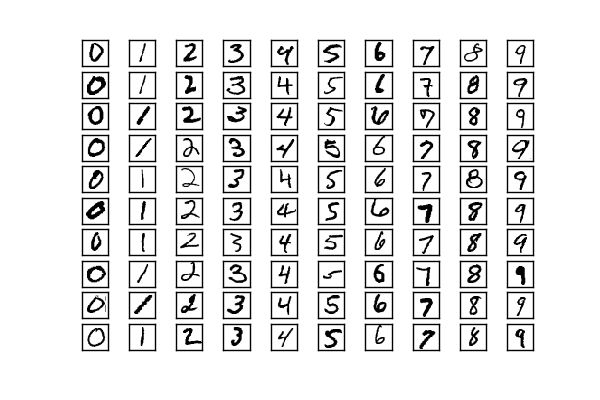
\includegraphics[scale=1.0]{Images/mnist}
	\caption{\label{fig:mnist_example} MNIST sample images having handwritten digits from 0-9, image size is 28x28 and images are grayscale, shown samples are randomly chosen, 10 for each class} 
\end{figure}


\subsection{CIFAR10}
MNIST dataset has50000 training samples and 10000 testing samples.It is database of different objects present in the images. Sample examples are shown in fig.\ref{fig:cifar10_example}

\begin{figure}[H]
	\centering
	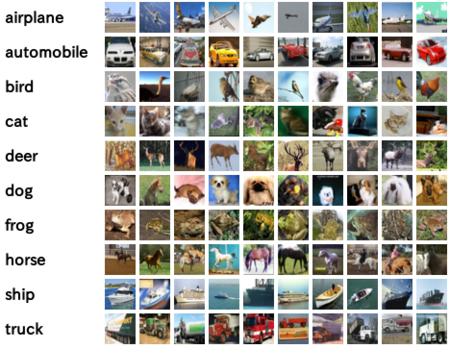
\includegraphics[scale=0.8]{Images/cifar10}
	\caption{\label{fig:cifar10_example} CIFAR-10 sample images having different objects present in the images, image size is 32x32 and images are color,} 
\end{figure}

\subsection{CIFAR100}
CIFAR100 dataset has 50000 training samples and 10000 testing samples.It is database of 100 different object classes. Sample examples are shown in fig.\ref{fig:cif00_example}

\begin{figure}[H]
	\centering
	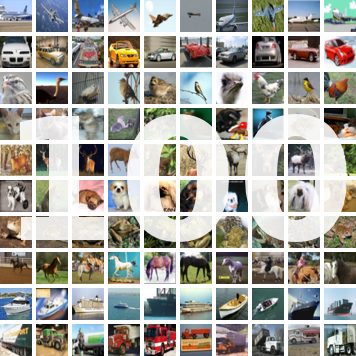
\includegraphics[scale=0.8]{Images/cifar_100}
	\caption{\label{fig:cif00_example} CIFAR-100 sample images consist of database with 100 different object classes, image size is 32x32 and images are color} 
\end{figure}

\subsection{Software}
Keras \cite{chollet2015} is mainly used for almost all the experiments. Theano \cite{2016arXiv160502688short} is used as main backend for Keras.Python is used as main programming language.